\documentclass[11pt,oneside]{article}

\pdfminorversion=7
\usepackage{PastProblemsStyle}

\hypersetup{
    pdftitle={Past Problems for Korean Undergraduate Mathematics Competition},
    pdfauthor={Jungwoo Kim},
    pdfsubject={Past problems for the Korean Undergraduate Mathematics Competition},
    pdfcreator={LaTeX}
}

\begin{document}

\thispagestyle{empty}

\begin{center}
    \vspace*{1.1cm}

    {\LARGE\bfseries Past Problems\par}

    \vspace{0.25cm}

    {\large for Korean Undergraduate Mathematics Competition\par}

    \vspace{0.75cm}

    {\normalsize
    Jungwoo Kim\\
    Department of Mathematics\\
    \PohangUniversityOfScienceAndTechnology
    \par}
\end{center}

\vspace{0.45cm}

\begin{sloppypar}
This document collects past problems from the Korean Undergraduate Mathematics \mbox{Competition}. General mathematical notation and writing follow \textit{(MATH000) Mathematical Language}.
\end{sloppypar}

\competitionyear{2001}

\begin{problem}{2001}{2}{1}
Let $0<a,b<1$ satisfy
\[
    \int_0^a\frac{1}{\sqrt{1-x^2}}\,\dd x
    =
    \int_b^1\frac{1}{\sqrt{1-x^2}}\,\dd x.
\]
Find $a^2+b^2$.
\end{problem}

\begin{problem}{2001}{2}{2}
For $n\times n$ matrices $\mathbf A,\mathbf B,\mathbf C$, prove that
\[
    \det
    \begin{pmatrix}
        \mathbf A & \mathbf B\\
        \mathbf C & \mathbf I_n
    \end{pmatrix}
    =
    \det(\mathbf A-\mathbf B\mathbf C),
\]
where $\mathbf I_n$ is the $n\times n$ identity matrix.
\end{problem}

\begin{problem}{2001}{2}{3}
Find the general solution of
\[
    y''-\frac1x y'-4x^2y=0,
    \qquad x>0.
\]
Hint: $y=e^{x^2}$ is a solution of the differential equation.
\end{problem}

\begin{problem}{2001}{2}{4}
Let $f\colon[0,\infty)\to[0,\infty)$ satisfy
\[
    2f(x)f(1)
    \le
    f(x)f(1)+1
    \le
    2f(2x)
\]
for every $x\ge0$. Prove that $f$ is constant.
\end{problem}

\begin{problem}{2001}{2}{5}
Let $f\colon[a,b]\to\R$ have a continuous derivative. Evaluate
\[
    \lim_{\lambda\to\infty}
    \int_a^b
    f(x)\left(|\sin(\lambda x)|-\frac2\pi\right)\,\dd x.
\]
\end{problem}

\begin{problem}{2001}{2}{6}
A triangle $ABC$ is inscribed in a circle of radius $1$. Let $a,b,c$ be the side lengths opposite the angles $A,B,C$, respectively. Find the maximum value of
\[
    a\cos A+b\cos B+c\cos C.
\]
\end{problem}

\begin{problem}{2001}{2}{7}
Evaluate the infinite series
\[
    \sum_{k=0}^{\infty}
    (-1)^k
    \left(\frac12\right)^{3k+2}
    \frac{9k+5}{(3k+1)(3k+2)}.
\]
\end{problem}

\begin{problem}{2001}{2}{8}
Let $(\mathbf v_1,\mathbf v_2,\dots,\mathbf v_n)$ be an orthonormal basis of $\R^n$, and let $\mathbf x\in\R^n$ be a unit vector. Prove that
\[
    \sum_{i=1}^n\|\mathbf x-\mathbf v_i\|^2
    \ge
    2n-2\sqrt n.
\]
Here $\|\mathbf v\|$ denotes the Euclidean norm of $\mathbf v$.
\end{problem}

\begin{problem}{2001}{2}{9}
Let $\lambda\ge0$ and $0<p<1$. Suppose $f$ is defined for $x>0$ and satisfies
\[
    f(x)=\bigl(x-\lambda f(x)\bigr)^p.
\]
Let $g(x)=x^p$. Prove that, for every $x>0$,
\[
    \frac{f'(x)}{g'(x)}<\frac1p.
\]
\end{problem}

\begin{problem}{2001}{1}{1}
Show that there are infinitely many triples $(a,b,c)\in\N^3$ satisfying
\[
    a\cos\left(\arctan\frac ba\right)
    +
    b\sin\left(\arctan\frac ba\right)
    =c.
\]
\end{problem}

\begin{problem}{2001}{1}{2}
For $n\times n$ matrices $\mathbf A,\mathbf B,\mathbf C$, prove that
\[
    \det
    \begin{pmatrix}
        \mathbf A & \mathbf B\\
        \mathbf C & \mathbf I_n
    \end{pmatrix}
    =
    \det(\mathbf A-\mathbf B\mathbf C),
\]
where $\mathbf I_n$ is the $n\times n$ identity matrix.
\end{problem}

\begin{problem}{2001}{1}{3}
Find the general solution of
\[
    y''-\frac1x y'-4x^2y=0,
    \qquad x>0.
\]
Hint: $y=e^{x^2}$ is a solution of the differential equation.
\end{problem}

\begin{problem}{2001}{1}{4}
Let $f\colon[0,\infty)\to[0,\infty)$ satisfy
\[
    2f(x)f(1)
    \le
    f(x)f(1)+1
    \le
    2f(2x)
\]
for every $x\ge0$. Prove that $f$ is constant.
\end{problem}

\begin{problem}{2001}{1}{5}
Evaluate
\[
    \lim_{n\to\infty}
    \int_0^{\pi/2}
    \frac{\sin x}{n^2\left(x-\frac\pi4\right)^2+1}\,\dd x.
\]
\end{problem}

\begin{problem}{2001}{1}{6}
A triangle $ABC$ is inscribed in a circle of radius $1$. Let $a,b,c$ be the side lengths opposite the angles $A,B,C$, respectively. Find the maximum value of
\[
    a\cos A+b\cos B+c\cos C.
\]
\end{problem}

\begin{problem}{2001}{1}{7}
Evaluate the infinite series
\[
    \sum_{k=0}^{\infty}
    (-1)^k
    \left(\frac12\right)^{3k+2}
    \frac{9k+5}{(3k+1)(3k+2)}.
\]
\end{problem}

\begin{problem}{2001}{1}{8}
Let $\mathbf v_1,\mathbf v_2,\dots,\mathbf v_n\in\R^2$ satisfy
\[
    \|\mathbf v_i\|\le1
    \qquad
    (i=1,2,\dots,n).
\]
Prove that there always exist signs
\[
    \varepsilon_1,\varepsilon_2,\dots,\varepsilon_n\in\{1,-1\}
\]
such that
\[
    \|\varepsilon_1\mathbf v_1+\varepsilon_2\mathbf v_2+\cdots+\varepsilon_n\mathbf v_n\|
    \le\sqrt2.
\]
Here $\|\mathbf v\|$ denotes the Euclidean norm of $\mathbf v$.
\end{problem}

\begin{problem}{2001}{1}{9}
Let $\lambda\ge0$ and $0<p<1$. Suppose $f$ is defined for $x>0$ and satisfies
\[
    f(x)=\bigl(x-\lambda f(x)\bigr)^p.
\]
Let $g(x)=x^p$. Prove that, for every $x>0$,
\[
    \frac{f'(x)}{g'(x)}<\frac1p.
\]
\end{problem}

\competitionyear{2002}

\begin{problem}{2002}{0}{1}
Let $f\colon\R\to\R$ be continuous. Suppose the function $x\mapsto xf(x)$ is differentiable for $x\ne0$ and
\[
    \frac{\dd}{\dd x}\bigl(xf(x)\bigr)=e^x.
\]
Find $f$.
\end{problem}

\begin{problem}{2002}{0}{2}
Let $(a_n)$ be an arithmetic sequence with first term $a$ and common difference $d$, and define the $2002\times2002$ matrix
\[
    \mathbf A\coloneqq
    \begin{pmatrix}
        a_1 & a_2 & a_3 & a_4 & \cdots & a_{2002}\\
        a_2 & a_1 & a_2 & a_3 & \cdots & a_{2001}\\
        a_3 & a_2 & a_1 & a_2 & \cdots & a_{2000}\\
        \vdots & \vdots & \vdots & \vdots & \ddots & \vdots\\
        a_{2002} & a_{2001} & a_{2000} & a_{1999} & \cdots & a_1
    \end{pmatrix}.
\]
Express $\det(\mathbf A)$ in terms of $a$ and $d$.
\end{problem}

\begin{problem}{2002}{0}{3}
Let $\mathbf a,\mathbf b,\mathbf c,\mathbf d$ be unit vectors in $\R^n$. Prove that
\[
    \left|
        \langle\mathbf a,\mathbf c\rangle
        \langle\mathbf b,\mathbf d\rangle
        -
        \langle\mathbf a,\mathbf d\rangle
        \langle\mathbf b,\mathbf c\rangle
    \right|
    \le1,
\]
where $\langle\cdot,\cdot\rangle$ denotes the standard inner product on $\R^n$.
\end{problem}

\begin{problem}{2002}{0}{4}
Let $n\in\N$, and let $a_1,\dots,a_n,x_1,\dots,x_n$ be positive real numbers satisfying
\begin{problemclauses}
    \item $a_1\le a_2\le\cdots\le a_n$;
    \item $x_k\ge x_n$ for $k=1,2,\dots,n-1$.
\end{problemclauses}
Prove that
\[
    (a_1+x_1a_2)(a_2+x_2a_3)\cdots
    (a_{n-1}+x_{n-1}a_n)(a_n+x_na_1)
    \ge
    a_1a_2\cdots a_n
    (x_1+1)(x_2+1)\cdots(x_n+1).
\]
\end{problem}

\begin{problem}{2002}{0}{5}
For $\alpha\in\C$, define the $n\times n$ matrix $\mathbf A_n=(a_{ij})$ by
\[
    a_{ij}
    =
    \begin{cases}
        1, & i=j,\\
        \alpha, & i-j=-1,\\
        \overline{\alpha}, & i-j=1,\\
        0, & |i-j|\ge2.
    \end{cases}
\]
Prove that $\mathbf A_n$ is positive semidefinite for every $n=1,2,\dots$ if and only if
\[
    |\alpha|\le\frac12.
\]
Here $\overline{\alpha}$ denotes the complex conjugate of $\alpha$.
\end{problem}

\begin{problem}{2002}{0}{6}
Solve the system of differential equations
\[
    x''(t)+2y'(t)-x(t)=0,
    \qquad
    y''(t)-2x'(t)-y(t)=0
\]
subject to
\[
    x(0)=y(0)=0,
    \qquad
    x'(0)=a>0,
    \qquad
    y'(0)=0.
\]
\end{problem}

\begin{problem}{2002}{2}{1}
For $(x,y)\ne(0,0)$, define
\[
    f(x,y)=\frac{x^2-xy+y^2}{2x^2+y^2}.
\]
Find the minimum value of $f$.
\end{problem}

\begin{problem}{2002}{2}{2}
Let $f,g,h\colon[-1,1]\to\R$ be continuous. Suppose that $f$ is odd, $g$ is even, and
\[
    \int_{-1}^{1}f(x)^2\,\dd x
    =
    \int_{-1}^{1}g(x)^2\,\dd x
    =1.
\]
Prove that
\[
    \left(\int_{-1}^{1}f(x)h(x)\,\dd x\right)^2
    +
    \left(\int_{-1}^{1}g(x)h(x)\,\dd x\right)^2
    \le
    \int_{-1}^{1}h(x)^2\,\dd x.
\]
\end{problem}

\begin{problem}{2002}{2}{3}
Let $a>b>0$. Evaluate
\[
    \int_0^{\infty}
    \frac{\arctan(ax)-\arctan(bx)}{x}\,\dd x.
\]
\end{problem}

\begin{problem}{2002}{1}{1}
Let $f\colon[a,b]\to\R$ have a continuous derivative, with $f(a)=0$. Suppose that
\[
    \left|\frac{f'(x)}{2003}\right|
    \le
    \left|\frac{f(x)}{2002}\right|
    \qquad
    (x\in[a,b]).
\]
Prove that $f(x)\equiv0$ on $[a,b]$.
\end{problem}

\begin{problem}{2002}{1}{2}
Let $n\in\N$ with $n>1$. Prove that
\[
    \frac{\bigl((n-1)!\bigr)^{1/(n-1)}}{(n!)^{1/n}}
    <
    \frac{(n!)^{1/n}}{\bigl((n+1)!\bigr)^{1/(n+1)}}.
\]
It is given that
\[
    4>e^{4-2\sqrt2}.
\]
\end{problem}

\begin{problem}{2002}{1}{3}
Let
\[
    \alpha=0.0110101000101000101\dots,
\]
where the $n$th digit after the decimal point is $1$ if $n$ is prime and $0$ otherwise. Prove that $\alpha$ is irrational.
\end{problem}

\competitionyear{2003}

\begin{problem}{2003}{2}{1}
Find the value of the natural number
\[
    \sum_{k=1}^{\infty}
    \binom{10^{10}}{\lfloor\log_{11}k\rfloor}.
\]
Here $\binom nr$ denotes the binomial coefficient and $\lfloor x\rfloor$ denotes the greatest integer not exceeding $x$.
\end{problem}

\begin{problem}{2003}{2}{2}
Four points $A,B,C,D$ are given in clockwise order on a fixed circle, and the quadrilateral $ABCD$ contains the center of the circle. Let $P,Q,R,S$ be the incenters of the triangles $ABC$, $BCD$, $CDA$, and $DAB$, respectively. Prove that $PQRS$ is a rectangle.
\end{problem}

\begin{problem}{2003}{2}{3}
Let $a,b\in\N$ and let $p,q$ be primes with $p<2003$ and $q<2003$. Find all ordered pairs
\[
    (p^a,q^b)
\]
satisfying
\[
    p^a-q^b=1.
\]
\end{problem}

\begin{problem}{2003}{2}{4}
Let $(x_n)$ be a sequence satisfying
\[
    0\le x_{n+1}\le x_n
\]
for every $n\in\N$, and suppose that
\[
    \sum_{n=1}^{\infty}x_n
\]
converges. Determine
\[
    \lim_{n\to\infty}n x_n.
\]
\end{problem}

\begin{problem}{2003}{2}{5}
Let $\mathbf x=(x_1,x_2,\dots,x_n)\in\R^n$ satisfy
\[
    x_1+x_2+\cdots+x_n=0.
\]
Prove that
\[
    \max_{1\le j\le n}|x_j|
    \le
    \left(\frac{n-1}{n}\right)^{1/2}\|\mathbf x\|_2,
\]
where
\[
    \|\mathbf x\|_2=(x_1^2+x_2^2+\cdots+x_n^2)^{1/2}.
\]
\end{problem}

\begin{problem}{2003}{2}{6}
For each $k=1,2,\dots,2002$, let $x_k$ be a real number satisfying
\[
    k-1\le x_k\le k.
\]
Define
\[
    B_k
    =
    \left\{
        \frac{2}{k}\sum_{i=1}^k|x-x_i|
        \,\middle|\,
        x\in\R
    \right\}
\]
and
\[
    A
    =
    \left\{
        \sum_{k=1}^{2002}y_k
        \,\middle|\,
        y_k\in B_k,\ k=1,2,\dots,2002
    \right\}.
\]
Prove that
\[
    \binom{2003}{2}\in A.
\]
\end{problem}

\begin{problem}{2003}{2}{7}
Prove that the real number $\sin 1$ is irrational.
\end{problem}

\begin{problem}{2003}{2}{8}
Let $f\colon[0,3]\to\R$ be continuous and suppose that
\[
    \int_0^3 x^k f(x)\,\dd x=0
    \qquad
    (k=0,1,2,\dots,n-1)
\]
and
\[
    \int_0^3 x^n f(x)\,\dd x=3.
\]
Prove that there exists an interval $A\subseteq[0,3]$ such that
\[
    |f(x)|\ge\left(\frac23\right)^n(n+1)
\]
for every $x\in A$.
\end{problem}

\begin{problem}{2003}{2}{9}
Let $f$ be the $2\pi$-periodic function defined by
\[
    f(x)=
    \begin{cases}
        \pi+x, & -\pi<x\le0,\\
        \pi-x, & 0<x\le\pi.
    \end{cases}
\]
Using the Fourier series of $f$, prove that
\[
    \frac{\pi^2}{8}
    =
    \frac1{1^2}+\frac1{3^2}+\cdots+\frac1{(2n-1)^2}+\cdots.
\]
\end{problem}

\begin{problem}{2003}{1}{1}
Find the value of the natural number
\[
    \sum_{k=1}^{\infty}
    \binom{10^{10}}{\lfloor\log_{11}k\rfloor}.
\]
Here $\binom nr$ denotes the binomial coefficient and $\lfloor x\rfloor$ denotes the greatest integer not exceeding $x$.
\end{problem}

\begin{problem}{2003}{1}{2}
Four points $A,B,C,D$ are given in clockwise order on a fixed circle, and the quadrilateral $ABCD$ contains the center of the circle. Let $P,Q,R,S$ be the incenters of the triangles $ABC$, $BCD$, $CDA$, and $DAB$, respectively. Prove that $PQRS$ is a rectangle.
\end{problem}

\begin{problem}{2003}{1}{3}
Let $a,b\in\N$ and let $p,q$ be primes with $p<2003$ and $q<2003$. Find all ordered pairs
\[
    (p^a,q^b)
\]
satisfying
\[
    p^a-q^b=1.
\]
\end{problem}

\begin{problem}{2003}{1}{4}
Let $(a_n)$ be a sequence with $a_n\ge0$ for every $n\in\N$, and suppose that
\[
    \sum_{n=1}^{\infty}a_n
\]
converges. Prove that, for every $p>\tfrac12$, the series
\[
    \sum_{n=1}^{\infty}\frac{\sqrt{a_n}}{n^p}
\]
converges. Also give an example showing that, when $p=\tfrac12$, the series
\[
    \sum_{n=1}^{\infty}\frac{\sqrt{a_n}}{n^p}
\]
may diverge.
\end{problem}

\begin{problem}{2003}{1}{5}
Let $p\ge1$ be a real number, and let $x_1,x_2,\dots,x_n>0$ satisfy
\[
    x_1+x_2+\cdots+x_n=1.
\]
Prove that
\[
    \sum_{j=1}^n\left(x_j+\frac1{x_j}\right)^p
    \ge
    \frac{(1+n^2)^p}{n^{p-1}}.
\]
\end{problem}

\begin{problem}{2003}{1}{6}
For each $k=1,2,\dots,2002$, let $x_k$ be a real number satisfying
\[
    k-1\le x_k\le k.
\]
Define
\[
    B_k
    =
    \left\{
        \frac{2}{k}\sum_{i=1}^k|x-x_i|
        \,\middle|\,
        x\in\R
    \right\}
\]
and
\[
    A
    =
    \left\{
        \sum_{k=1}^{2002}y_k
        \,\middle|\,
        y_k\in B_k,\ k=1,2,\dots,2002
    \right\}.
\]
Prove that
\[
    \binom{2003}{2}\in A.
\]
\end{problem}

\begin{problem}{2003}{1}{7}
Prove that the real number $\sin 1$ is irrational.
\end{problem}

\begin{problem}{2003}{1}{8}
Let $f\colon[0,3]\to\R$ be continuous and suppose that
\[
    \int_0^3 x^k f(x)\,\dd x=0
    \qquad
    (k=0,1,2,\dots,n-1)
\]
and
\[
    \int_0^3 x^n f(x)\,\dd x=3.
\]
Prove that there exists an interval $A\subseteq[0,3]$ such that
\[
    |f(x)|\ge\left(\frac23\right)^n(n+1)
\]
for every $x\in A$.
\end{problem}

\begin{problem}{2003}{1}{9}
Let $\mathbf A=(a_{ij})$ be an $n\times n$ matrix whose entries are all $0$ or $1$. Suppose that, for some $t\in\N$,
\[
    \mathbf A\mathbf A^{\mathsf T}
    =
    \begin{pmatrix}
        t+1 & 1 & \cdots & 1 & 1\\
        1 & t+1 & \cdots & 1 & 1\\
        \vdots & \vdots & \ddots & \vdots & \vdots\\
        1 & 1 & \cdots & t+1 & 1\\
        1 & 1 & \cdots & 1 & t+1
    \end{pmatrix}
    =t\mathbf I_n+\mathbf J,
\]
where $\mathbf A^{\mathsf T}$ denotes the transpose of $\mathbf A$, $\mathbf I_n$ is the $n\times n$ identity matrix, and $\mathbf J$ is the $n\times n$ all-ones matrix. Express $\det(\mathbf A)$ as a function of $t$.
\end{problem}

\competitionyear{2004}

\begin{problem}{2004}{2}{1}
Let $f\colon\R\to\R$ satisfy
\[
    f(x+y)=f(x)+f(y)
\]
for all $x,y\in\R$. Prove the following.
\begin{problemsubparts}
    \item If $f$ is continuous at $0$, then $f$ is continuous at every $x\in\R$.
    \item If $f$ is continuous on $\R$ and $f(1)=c$, then $f(x)=cx$ for every $x\in\R$.
\end{problemsubparts}
\end{problem}

\begin{problem}{2004}{2}{2}
A frustum of a pyramid has parallel upper and lower bases and uniform density. Find the ratio of the distance from its center of mass to the lower base to the distance from its center of mass to the upper base. The similarity ratio of the upper base to the lower base is $r$, where $r<1$.
\begin{center}
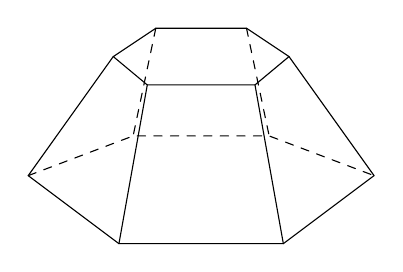
\begin{tikzpicture}[scale=0.72,line cap=round,line join=round]
    \coordinate (T1) at (-1.55,1.55);
    \coordinate (T2) at (-0.80,2.05);
    \coordinate (T3) at (0.80,2.05);
    \coordinate (T4) at (1.55,1.55);
    \coordinate (T5) at (0.95,1.05);
    \coordinate (T6) at (-0.95,1.05);

    \coordinate (B1) at (-3.05,-0.55);
    \coordinate (B2) at (-1.20,0.15);
    \coordinate (B3) at (1.20,0.15);
    \coordinate (B4) at (3.05,-0.55);
    \coordinate (B5) at (1.45,-1.75);
    \coordinate (B6) at (-1.45,-1.75);

    \draw (T1)--(T2)--(T3)--(T4)--(T5)--(T6)--cycle;

    \draw (T1)--(B1);
    \draw[dashed] (T2)--(B2);
    \draw[dashed] (T3)--(B3);
    \draw (T4)--(B4);
    \draw (T5)--(B5);
    \draw (T6)--(B6);

    \draw[dashed] (B1)--(B2)--(B3)--(B4);
    \draw (B4)--(B5)--(B6)--(B1);
\end{tikzpicture}
\end{center}

\end{problem}

\begin{problem}{2004}{2}{3}
A convex quadrilateral $ABCD$ has side lengths $a,b,c,d$, in this order starting from $AB$. Show that if its area is maximal among all such quadrilaterals, then $ABCD$ is cyclic.
\end{problem}

\begin{problem}{2004}{2}{4}
Let $(\mathbf v_1,\mathbf v_2,\dots,\mathbf v_n)$ be an orthonormal basis of $\R^n$. Find the orthogonal complement of
\[
    \Span\{i\mathbf v_i-j\mathbf v_j\mid 1\le i<j\le n\}.
\]
\end{problem}

\begin{problem}{2004}{2}{5}
Let $f\colon[a,c]\to(0,\infty)$ be continuous on $[a,c]$ and differentiable on $(a,c)$. Let
\[
    P=(x_0,f(x_0))
\]
be a point on the graph of $f$. Let $\alpha$ and $\gamma$ be the angles made with the $x$-axis by the lines joining $P$ to $(a,0)$ and $(c,0)$, respectively, and let $\beta$ be the angle made with the $x$-axis by the tangent line to the graph at $P$. Show that there exists $x_0\in(a,c)$ such that
\[
    \tan\alpha+\tan\beta+\tan\gamma=0.
\]
If the tangent line does not meet the $x$-axis, take $\beta=0$.
\end{problem}

\begin{problem}{2004}{2}{6}
Let $f\colon\R\to\R$ be a function whose second derivative $f''$ exists and is bounded on $[0,1]$. Let $(a_n)$ be a sequence such that $0<a_n<1$ for every $n\in\N$, the series
\[
    \sum_{n=1}^{\infty}a_n
\]
diverges, and the series
\[
    \sum_{n=1}^{\infty}a_n^2
\]
converges. If
\[
    \sum_{n=1}^{\infty}f(a_n)
\]
converges, prove that
\[
    \sum_{n=1}^{\infty}|f(a_n)|
\]
also converges.
\end{problem}

\begin{problem}{2004}{2}{7}
Suppose a plane curve $(x(t),y(t))$ of period $T$ satisfies
\[
    \frac{\dd x}{\dd t}=ax-bxy,
    \qquad
    \frac{\dd y}{\dd t}=-cy+dxy,
    \qquad
    x(0)=y(0)=1,
\]
where $a,b,c,d>0$. Find
\[
    \overline{x}\coloneqq\frac1T\int_0^T x(t)\,\dd t,
    \qquad
    \overline{y}\coloneqq\frac1T\int_0^T y(t)\,\dd t.
\]
\end{problem}

\begin{problem}{2004}{2}{8}
Evaluate
\[
    \int_0^{\pi}\frac{x\sin x}{1+\cos^2x}\,\dd x.
\]
\end{problem}

\begin{problem}{2004}{2}{9}
Let $B$ be any $30$-element subset of $\{1,2,\dots,39,40\}$. Prove that there exists a subset $A\subseteq B$ such that
\begin{problemclauses}
    \item $|A|\ge10$;
    \item $x+y\notin A$ for all $x,y\in A$.
\end{problemclauses}
\end{problem}

\begin{problem}{2004}{1}{1}
Let $f\colon\R\to\R$ satisfy
\[
    f(x+y)=f(x)+f(y)
\]
for all $x,y\in\R$. Prove the following.
\begin{problemsubparts}
    \item If $f$ is continuous at $0$, then $f$ is continuous at every $x\in\R$.
    \item If $f$ is continuous on $\R$ and $f(1)=c$, then $f(x)=cx$ for every $x\in\R$.
\end{problemsubparts}
\end{problem}

\begin{problem}{2004}{1}{2}
A frustum of a pyramid has parallel upper and lower bases and uniform density. Find the ratio of the distance from its center of mass to the lower base to the distance from its center of mass to the upper base. The similarity ratio of the upper base to the lower base is $r$, where $r<1$.
\begin{center}
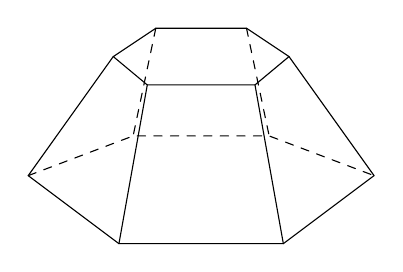
\begin{tikzpicture}[scale=0.72,line cap=round,line join=round]
    \coordinate (T1) at (-1.55,1.55);
    \coordinate (T2) at (-0.80,2.05);
    \coordinate (T3) at (0.80,2.05);
    \coordinate (T4) at (1.55,1.55);
    \coordinate (T5) at (0.95,1.05);
    \coordinate (T6) at (-0.95,1.05);

    \coordinate (B1) at (-3.05,-0.55);
    \coordinate (B2) at (-1.20,0.15);
    \coordinate (B3) at (1.20,0.15);
    \coordinate (B4) at (3.05,-0.55);
    \coordinate (B5) at (1.45,-1.75);
    \coordinate (B6) at (-1.45,-1.75);

    \draw (T1)--(T2)--(T3)--(T4)--(T5)--(T6)--cycle;

    \draw (T1)--(B1);
    \draw[dashed] (T2)--(B2);
    \draw[dashed] (T3)--(B3);
    \draw (T4)--(B4);
    \draw (T5)--(B5);
    \draw (T6)--(B6);

    \draw[dashed] (B1)--(B2)--(B3)--(B4);
    \draw (B4)--(B5)--(B6)--(B1);
\end{tikzpicture}
\end{center}

\end{problem}

\begin{problem}{2004}{1}{3}
A convex quadrilateral $ABCD$ has side lengths $a,b,c,d$, in this order starting from $AB$. Show that if its area is maximal among all such quadrilaterals, then $ABCD$ is cyclic.
\end{problem}

\begin{problem}{2004}{1}{4}
Let $(\mathbf v_1,\mathbf v_2,\dots,\mathbf v_n)$ be an orthonormal basis of $\R^n$. Find the orthogonal complement of
\[
    \Span\{i\mathbf v_i-j\mathbf v_j\mid 1\le i<j\le n\}.
\]
\end{problem}

\begin{problem}{2004}{1}{5}
Let $A$ be the least positive integer of the form
\[
    33^k-7^\ell,
    \qquad k,\ell\in\N,
\]
and let $B$ be the least positive integer of the form
\[
    7^m-33^n,
    \qquad m,n\in\N.
\]
Find $A+B$.
\end{problem}

\begin{problem}{2004}{1}{6}
Let $f\colon\R\to\R$ be a function whose second derivative $f''$ exists and is bounded on $[0,1]$. Let $(a_n)$ be a sequence such that $0<a_n<1$ for every $n\in\N$, the series
\[
    \sum_{n=1}^{\infty}a_n
\]
diverges, and the series
\[
    \sum_{n=1}^{\infty}a_n^2
\]
converges. If
\[
    \sum_{n=1}^{\infty}f(a_n)
\]
converges, prove that
\[
    \sum_{n=1}^{\infty}|f(a_n)|
\]
also converges.
\end{problem}

\begin{problem}{2004}{1}{7}
Suppose a plane curve $(x(t),y(t))$ of period $T$ satisfies
\[
    \frac{\dd x}{\dd t}=ax-bxy,
    \qquad
    \frac{\dd y}{\dd t}=-cy+dxy,
    \qquad
    x(0)=y(0)=1,
\]
where $a,b,c,d>0$. Find
\[
    \overline{x}\coloneqq\frac1T\int_0^T x(t)\,\dd t,
    \qquad
    \overline{y}\coloneqq\frac1T\int_0^T y(t)\,\dd t.
\]
\end{problem}

\begin{problem}{2004}{1}{8}
Let $\mathbf v\in\R^n$ be a unit vector, and let $\mathbf P_{\mathbf v}$ denote the orthogonal projection onto the line $\Span(\mathbf v)$, so that
\[
    \mathbf P_{\mathbf v}\mathbf x=(\mathbf x\cdot\mathbf v)\mathbf v
\]
for every $\mathbf x\in\R^n$. Let $\mathbf A$ be an $n\times n$ positive definite symmetric matrix. Find the maximum value of $\lambda$ such that
\[
    \mathbf A-\lambda\mathbf P_{\mathbf v}\succeq0.
\]
Here $\mathbf B\succ0$ means that every eigenvalue of the symmetric matrix $\mathbf B$ is positive, and $\mathbf B\succeq0$ means that every eigenvalue is nonnegative.
\end{problem}

\begin{problem}{2004}{1}{9}
Let $B$ be any $30$-element subset of $\{1,2,\dots,39,40\}$. Prove that there exists a subset $A\subseteq B$ such that
\begin{problemclauses}
    \item $|A|\ge10$;
    \item $x+y\notin A$ for all $x,y\in A$.
\end{problemclauses}
\end{problem}

\competitionyear{2005}

\begin{problem}{2005}{0}{1}
Let
\[
    \mathbf A=\frac12
    \begin{pmatrix}
        0 & \sqrt2\\
        -\sqrt2 & 0
    \end{pmatrix}.
\]
Find the matrix
\[
    e^{\mathbf A}=\sum_{n=0}^{\infty}\frac{\mathbf A^n}{n!}.
\]
\end{problem}

\begin{problem}{2005}{0}{2}
Solve the differential equation
\[
    y'(t)+2t y(t)=t y(t)^2,
    \qquad
    y(1)=1.
\]
\end{problem}

\begin{problem}{2005}{0}{3}
Let $p\ge3$ be an arbitrary prime, and let
\[
    \mathbb F_p=\{0,1,\dots,p-1\}.
\]
Show that the set
\[
    S=\{(x,y)\in\mathbb F_p^2\mid x^2+y^2\equiv-1\pmod p\}
\]
is nonempty.
\end{problem}

\begin{problem}{2005}{0}{4}
Let $f\colon\R\to\R$ be differentiable and suppose that
\[
    |f(n)|\le\frac1{(1+n)^{5/4}}
\]
for every nonnegative integer $n$, and that
\[
    |f'(x)|\le e^{-x}
\]
for every $x\in\R$. Prove that
\[
    \int_0^{\infty}|f(x)|\,\dd x<\infty.
\]
\end{problem}

\begin{problem}{2005}{0}{5}
Let $S_n$ be the set of all bijections from $\{1,2,\dots,n\}$ to itself. For $\sigma\in S_n$, let $f(\sigma)$ denote the number of fixed points of $\sigma$, that is,
\[
    f(\sigma)=|\{x\in\{1,2,\dots,n\}\mid \sigma(x)=x\}|.
\]
Find
\[
    \sum_{\sigma\in S_n} f(\sigma).
\]
\end{problem}

\begin{problem}{2005}{2}{1}
A population consists of smokers and nonsmokers. Each year, $5\%$ of the nonsmokers begin smoking and $10\%$ of the smokers quit smoking. Prove that, after a sufficiently long time, the ratio of smokers to nonsmokers converges to a constant, and find that ratio.
\end{problem}

\begin{problem}{2005}{2}{2}
Let $X$ be the set of all invertible $2\times2$ matrices and $Y$ the set of all invertible $3\times3$ matrices. Define $\Phi\colon X\to Y$ by
\[
    \Phi\left(
    \begin{pmatrix}
        a&b\\
        c&d
    \end{pmatrix}
    \right)
    =
    \begin{pmatrix}
        a^2&2ab&b^2\\
        ac&ad+bc&bd\\
        c^2&2cd&d^2
    \end{pmatrix}.
\]
Suppose $\mathbf A\in X$ has eigenvalues $1,x$ and $\mathbf B\in X$ has eigenvalues $1+x,1-x$. Find
\[
    \det\bigl(\Phi(\mathbf A\mathbf B)\bigr).
\]
\end{problem}

\begin{problem}{2005}{2}{3}
Words of length $n$ are formed using the three letters $A,B,C$, with the restriction that $A$ may not occur twice consecutively. Express the number of such words as a function of $n$.
\end{problem}

\begin{problem}{2005}{2}{4}
Let $f\colon(0,\infty)\to\R$ be twice differentiable and suppose that
\[
    |f(x)|\le1,
    \qquad
    |f''(x)|\le1
\]
for every $x\in(0,\infty)$. Prove that
\[
    |f'(x)|\le2
\]
for every $x\in(0,\infty)$.
\end{problem}

\begin{problem}{2005}{1}{1}
A population consists of smokers and nonsmokers. Each year, $5\%$ of the nonsmokers begin smoking and $10\%$ of the smokers quit smoking. Prove that, after a sufficiently long time, the ratio of smokers to nonsmokers converges to a constant, and find that ratio.
\end{problem}

\begin{problem}{2005}{1}{2}
Let $f\colon[0,1]\to\R$ be differentiable, with $f(0)=0$ and $f(1)=1$. Prove that, for every $n\in\N$, there exist distinct points $x_1,x_2,\dots,x_n\in[0,1]$ such that
\[
    \sum_{k=1}^{n}\frac1{f'(x_k)}=n.
\]
\end{problem}

\begin{problem}{2005}{1}{3}
Words of length $n$ are formed using the three letters $A,B,C$, with the restriction that $A$ may not occur twice consecutively. Express the number of such words as a function of $n$.
\end{problem}

\begin{problem}{2005}{1}{4}
Let $(a_n)$ and $(b_n)$ be sequences satisfying $a_n>0$ and $b_n>0$ for every $n\in\N$, and suppose that
\[
    \sum_{n=1}^{\infty}a_n=3,
    \qquad
    \sum_{n=1}^{\infty}b_n=4.
\]
Find the supremum and infimum of all possible values of
\[
    \sum_{n=1}^{\infty}\frac{a_n^2}{a_n+b_n}.
\]
\end{problem}

\competitionyear{2006}

\begin{problem}{2006}{0}{1}
Let $f(x)=\arctan(2x)$. Find $f^{(99)}(0)$.
\end{problem}

\begin{problem}{2006}{0}{2}
Let $f\colon\R\to\R$ be a continuous periodic function with period $2T$. Prove that there exists a suitable $x_0\in\R$ such that
\[
    f(x_0+T)=f(x_0).
\]
\end{problem}

\begin{problem}{2006}{0}{3}
Let $\mathbf A$ be an $n\times n$ matrix such that
\[
    \tr(\mathbf X\mathbf Y\mathbf A)=\tr(\mathbf Y\mathbf X\mathbf A)
\]
for every pair of $n\times n$ matrices $\mathbf X,\mathbf Y$. Prove that $\mathbf A$ is a scalar multiple of the identity matrix. Here $\tr$ denotes the sum of the diagonal entries.
\end{problem}

\begin{problem}{2006}{0}{4}
Let $(a_n)$ be a sequence of positive real numbers, and suppose that the limit
\[
    \lim_{n\to\infty}n\left(\frac{a_n}{a_{n+1}}-1\right)
\]
exists. Prove that if this limit is greater than $1$, then the series
\[
    \sum_{n=1}^{\infty}a_n
\]
converges.
\end{problem}

\begin{problem}{2006}{0}{5}
Let $f\colon(0,\infty)\to\R$ be differentiable, suppose that $f'$ is continuous, and assume that
\[
    \lim_{x\to\infty}\bigl(f(x)+f'(x)\bigr)=0.
\]
Prove that
\[
    \lim_{x\to\infty}f(x)=0.
\]
\end{problem}

\begin{problem}{2006}{2}{1}
Evaluate
\[
    \int_{-\pi}^{\pi}\ln\left|\sin\frac{\theta}{2}\right|\,\dd\theta.
\]
\end{problem}

\begin{problem}{2006}{2}{2}
Let $\mathbf a=(a_1,a_2,\dots,a_n)$ be a unit vector, and let $\mathbf X=(x_{ij})$ be the $n\times n$ matrix defined by
\[
    x_{ij}=\delta_{ij}+a_i a_j,
\]
where $\delta_{ij}=1$ if $i=j$ and $\delta_{ij}=0$ if $i\ne j$. Compute $\det(\mathbf X)$.
\end{problem}

\begin{problem}{2006}{2}{3}
Let $h\colon\R\to\R$ satisfy
\[
    \int_0^{\infty}h(t)\,\dd t=1.
\]
Evaluate
\[
    \iint_{\R^2}h(x^2+2xy+5y^2)\,\dd A.
\]
\end{problem}

\begin{problem}{2006}{2}{4}
Evaluate the series
\[
    1-\frac15+\frac17-\frac1{11}+\cdots
    +\frac1{6n-5}-\frac1{6n-1}+\cdots.
\]
\end{problem}

\begin{problem}{2006}{1}{1}
Prove that the improper integral
\[
    \int_0^{\infty}\sin(x^2)\,\dd x
\]
converges, whereas
\[
    \int_0^{\infty}|\sin(x^2)|\,\dd x
\]
diverges.
\end{problem}

\begin{problem}{2006}{1}{2}
Let $\mathbf a=(a_1,a_2,\dots,a_n)$ be a unit vector, and let $\mathbf X=(x_{ij})$ be the $n\times n$ matrix defined by
\[
    x_{ij}=\delta_{ij}+a_i a_j,
\]
where $\delta_{ij}=1$ if $i=j$ and $\delta_{ij}=0$ if $i\ne j$. Compute $\det(\mathbf X)$.
\end{problem}

\begin{problem}{2006}{1}{3}
Let $h\colon\R\to\R$ satisfy
\[
    \int_0^{\infty}h(t)\,\dd t=1.
\]
Evaluate
\[
    \iint_{\R^2}h(x^2+2xy+5y^2)\,\dd A.
\]
\end{problem}

\begin{problem}{2006}{1}{4}
Consider the alternating harmonic series
\[
    1-\frac12+\frac13-\frac14+\frac15-\cdots.
\]
Let $\sum a_k$ be a series obtained by rearranging its terms subject to the rule that the relative order among terms of the same sign is not changed. For example,
\[
    1+\frac13-\frac12-\frac14+\cdots
\]
is allowed, whereas
\[
    1-\frac14+\frac13-\frac12+\cdots
\]
is not. Among $a_1,a_2,\dots,a_n$, let $p_n$ be the number of positive terms and $q_n$ the number of negative terms.
\begin{problemsubparts}
    \item Prove that $\sum a_k$ converges if and only if the limit
    \[
        \lim_{n\to\infty}\frac{p_n}{q_n}
    \]
    exists.
    \item If this limit is $\alpha$, prove that
    \[
        \sum a_k=\ln2+\frac12\ln\alpha.
    \]
\end{problemsubparts}
\end{problem}

\competitionyear{2007}

\begin{problem}{2007}{2}{1}
Evaluate
\[
    \int_0^1\int_0^x(3-x-y)\,\dd y\,\dd x.
\]
\end{problem}

\begin{problem}{2007}{2}{2}
Let $C(t)=(\cos t,\sin t)$ for $0\le t\le2\pi$. Evaluate the line integral
\[
    \int_C\frac{y\,\dd x-x\,\dd y}{x^2+y^2}.
\]
\end{problem}

\begin{problem}{2007}{2}{3}
Find the area of the quadrilateral whose vertices are
\[
    (0,0,0),\quad(1,2,3),\quad(3,1,2),\quad(7,4,7).
\]
\end{problem}

\begin{problem}{2007}{2}{4}
Let
\[
    f(x)=\frac{e^x}{x},
    \qquad 1\le x\le2,
\]
and let $g$ be the inverse function of $f$. Evaluate
\[
    \int_e^{e^2/2}[g(x)]^2\,\dd x.
\]
\end{problem}

\begin{problem}{2007}{2}{5}
Find the functions $x(t)$ and $y(t)$ satisfying
\[
    x'(t)=-y(t),
    \qquad
    y'(t)=x(t),
    \qquad
    (x(0),y(0))=(1,1).
\]
\end{problem}

\begin{problem}{2007}{2}{6}
Find the relation among $a,b,c$ that is necessary and sufficient for the system
\[
\begin{aligned}
    x_1-2x_2-x_3+3x_4&=a,\\
    2x_1+4x_2+6x_3-2x_4&=b,\\
    x_1+x_3+x_4&=c
\end{aligned}
\]
to have a solution.
\end{problem}

\begin{problem}{2007}{2}{7}
Write the matrix
\[
    \begin{pmatrix}
        1&-3&0\\
        0&1&3\\
        2&-10&2
    \end{pmatrix}
\]
as $\mathbf L\mathbf U$, where $\mathbf L$ is lower triangular and $\mathbf U$ is upper triangular.
\end{problem}

\begin{problem}{2007}{2}{8}
Three unit vectors $\mathbf v_1,\mathbf v_2,\mathbf v_3\in\R^3$ determine a parallelepiped of volume $\tfrac12$. Let $\theta_{ij}$ be the angle between $\mathbf v_i$ and $\mathbf v_j$, and let $\mathbf A$ be the $3\times3$ matrix whose $(i,j)$-entry is $\cos\theta_{ij}$. Compute $\det(\mathbf A)$.
\end{problem}

\begin{problem}{2007}{2}{9}
Find the volume of the region in $\R^3$ described by
\[
    x=(p-q)\cos t,
    \qquad
    y=(p-q)\sin t,
    \qquad
    z=p+q,
\]
where
\[
    0\le t\le2\pi,
    \qquad
    1-\varepsilon\le p\le1+\varepsilon,
    \qquad
    -\delta\le q\le\delta,
    \qquad
    \delta<1-\varepsilon.
\]
\end{problem}

\begin{problem}{2007}{2}{10}
Find the constants $a,b$ that minimize
\[
    \int_0^{\pi}[\sin x-(ax+b)]^2\,\dd x.
\]
\end{problem}

\begin{problem}{2007}{2}{11}
Let $\mathbf v_1,\mathbf v_2,\mathbf v_3\in\R^3$ be linearly independent vectors satisfying
\[
    \|\mathbf v_i\|=1,
    \qquad
    \mathbf v_i\cdot\mathbf v_j=-\frac13
    \quad(i\ne j).
\]
For vectors $\mathbf x\in\R^3$ with $\|\mathbf x\|=1$, find the maximum and minimum values of
\[
    \sum_{i=1}^3\|\mathbf x-\mathbf v_i\|^2.
\]
\end{problem}

\begin{problem}{2007}{2}{12}
For real $y$, evaluate
\[
    \int_{-\infty}^{\infty}\frac{e^{-2\pi i yx}}{\cosh(\pi x)}\,\dd x.
\]
\end{problem}

\begin{problem}{2007}{2}{13}
Let $p>0$ be real. Evaluate
\[
    \lim_{n\to\infty}
    \frac1{n^2}
    \sum_{k=1}^{n}
    \left(1^p+2^p+3^p+\cdots+k^p\right)^{1/(p+1)}.
\]
\end{problem}

\begin{problem}{2007}{1}{1}
Find the area of the quadrilateral whose vertices are
\[
    (0,0,0),\quad(1,2,3),\quad(3,1,2),\quad(7,4,7).
\]
\end{problem}

\begin{problem}{2007}{1}{2}
Let
\[
    f(x)=\frac{e^x}{x},
    \qquad 1\le x\le2,
\]
and let $g$ be the inverse function of $f$. Evaluate
\[
    \int_e^{e^2/2}[g(x)]^2\,\dd x.
\]
\end{problem}

\begin{problem}{2007}{1}{3}
Let $A=\{1,2,3,\dots,n\}$. Suppose $k$ distinct subsets of $A$, each containing exactly $\gamma$ elements, are selected. Prove that if every element of $A$ is to belong to at least $p$ of the selected subsets, then
\[
    k\ge\frac{np}{\gamma}.
\]
\end{problem}

\begin{problem}{2007}{1}{4}
Three unit vectors $\mathbf v_1,\mathbf v_2,\mathbf v_3\in\R^3$ determine a parallelepiped of volume $\tfrac12$. Let $\theta_{ij}$ be the angle between $\mathbf v_i$ and $\mathbf v_j$, and let $\mathbf A$ be the $3\times3$ matrix whose $(i,j)$-entry is $\cos\theta_{ij}$. Compute $\det(\mathbf A)$.
\end{problem}

\begin{problem}{2007}{1}{5}
Let $M_{2\times2}$ be the vector space of $2\times2$ matrices, and let $\mathbf T\in M_{2\times2}$ be invertible. Compute the determinant of the linear map
\[
    \Phi\colon M_{2\times2}\to M_{2\times2},
    \qquad
    \Phi(\mathbf A)=\mathbf T\mathbf A\mathbf T^{-1}.
\]
\end{problem}

\begin{problem}{2007}{1}{6}
In triangle $ABC$, let $P$ be a point on the side $BC$. Put
\[
    BP=x,
    \qquad
    BC=l,
\]
let the altitude of the triangle be $h$, and let
\[
    \angle APC=\theta(x).
\]
Prove that
\[
    \angle A=\frac1h\int_0^l\sin^2\theta(x)\,\dd x.
\]
\end{problem}

\begin{problem}{2007}{1}{7}
Let $\mathbf A$ and $\mathbf B$ be real matrices. Suppose there exists a complex matrix $\mathbf S$ such that
\[
    \mathbf A=\mathbf S^{-1}\mathbf B\mathbf S.
\]
Prove that there exists a real matrix $\mathbf R$ such that
\[
    \mathbf A=\mathbf R^{-1}\mathbf B\mathbf R.
\]
\end{problem}

\begin{problem}{2007}{1}{8}
Let $a_1>0$ and
\[
    a_{n+1}=\ln(1+a_n).
\]
Prove that
\[
    \lim_{n\to\infty}n a_n=2.
\]
\end{problem}

\begin{problem}{2007}{1}{9}
Let $(a_n)$ be a sequence such that
\[
    \sum_{n=1}^{\infty}a_n=1.
\]
Prove that
\[
    \lim_{n\to\infty}
    \sum_{k=1}^{n}a_k\left(1-\frac{k^2}{n^2}\right)=1.
\]
\end{problem}

\begin{problem}{2007}{1}{10}
Let $F\colon\R^2\to\R^2$ satisfy the following condition: for every triangle $\Delta$ of area $1$, $F(\Delta)$ is also a triangle of area $1$. Prove that for every straight line $l$, $F(l)$ is also a straight line.
\end{problem}

\competitionyear{2008}

\begin{problem}{2008}{2}{1}
Find the volume of the tetrahedron whose vertices are
\[
    (0,1,0),\quad(1,2,1),\quad(1,3,3),\quad(3,1,2).
\]
\end{problem}

\begin{problem}{2008}{2}{2}
Evaluate
\[
    \int_0^{\infty}\frac{e^{-x}-e^{-2x}}{x}\,\dd x.
\]
\end{problem}

\begin{problem}{2008}{2}{3}
Evaluate
\[
    \int_0^{\sqrt{\pi/2}}
    \int_0^{\sqrt{\pi/2}}
    \int_0^{\sqrt{\pi/2}}
    xyz\cos(x^2+y^2+z^2)\,\dd x\,\dd y\,\dd z.
\]
\end{problem}

\begin{problem}{2008}{2}{4}
Let $\alpha>1$. Prove that the improper integral
\[
    \int_1^{\infty}\cos(x^\alpha)\,\dd x
\]
converges.
\end{problem}

\begin{problem}{2008}{2}{5}
Find one matrix $\mathbf A$ satisfying
\[
    \mathbf A^2=
    \begin{pmatrix}
        2&-1\\
        -1&2
    \end{pmatrix}.
\]
\end{problem}

\begin{problem}{2008}{2}{6}
Find a function $f(x,y,z)$ satisfying
\[
    \nabla f(x,y,z)
    =
    \left(
        ye^{xy+yz},
        (x+z)e^{xy+yz},
        ye^{xy+yz}
    \right).
\]
\end{problem}

\begin{problem}{2008}{2}{7}
Find the maximum value of
\[
    f(x,y)=3x^2+4xy+y^2
\]
on the set
\[
    \{(x,y)\in\R^2\mid x^2+y^2=1\}.
\]
\end{problem}

\begin{problem}{2008}{2}{8}
Find all $3\times1$ column vectors $\mathbf u$ and $\mathbf v$ satisfying
\[
    \begin{pmatrix}
        5&2&3\\
        15&6&9\\
        10&4&6
    \end{pmatrix}
    =\mathbf u\mathbf v^{\mathsf T}.
\]
\end{problem}

\begin{problem}{2008}{2}{9}
Let $\mathbf A=(a_{ij})$ be an $n\times n$ matrix satisfying
\[
    \sum_{i=1}^{n}a_{ij}=0
\]
for every $j=1,2,\dots,n$. Prove that $\mathbf A$ is not invertible.
\end{problem}

\begin{problem}{2008}{2}{10}
Let $(\phi_n)$ be a sequence of functions defined on $[0,1]$ satisfying
\begin{problemsubparts}
    \item $\phi_0(t)=0$;
    \item
    \[
        \phi_n(t)
        =1+2\sin\frac t2
        -\frac12\int_0^t\phi_{n-1}(s)\,\dd s,
        \qquad n=1,2,\dots.
    \]
\end{problemsubparts}
Suppose that $\phi_n\to\phi$ on $[0,1]$ and that $\phi$ is differentiable. Find $\phi(t)$.
\end{problem}

\begin{problem}{2008}{2}{11}
Find all polynomial functions $u(x,y)$ satisfying the following conditions.
\begin{problemsubparts}
    \item $u_{xx}+u_{yy}=0$.
    \item For every $x\in\R$,
    \[
        u(x,0)=u(x,\sqrt3\,x)=0.
    \]
    \item For every $x>0$ and $0<y<\sqrt3\,x$,
    \[
        u(x,y)>0.
    \]
    \item There exists a positive integer $n$ such that, for every $t\in\R$,
    \[
        u(tx,ty)=t^n u(x,y).
    \]
\end{problemsubparts}
\end{problem}

\begin{problem}{2008}{2}{12}
For every $n=0,1,2,3,\dots$, let $a_n$ be either $0$ or $1$. Let $P$ and $Q$ be polynomials with $\deg P<\deg Q$, and suppose that for $|x|<1$,
\[
    \sum_{n=0}^{\infty}a_nx^n=\frac{P(x)}{Q(x)}.
\]
Prove that there exists a positive integer $p$ such that
\[
    a_{n+p}=a_n
\]
for every $n\ge0$.
\end{problem}

\begin{problem}{2008}{2}{13}
For the four data points
\[
    (0,0),\quad(1,1),\quad(3,2),\quad(4,5),
\]
find the line $y=ax+b$ that minimizes the sum of squared errors
\[
    E^2=\sum_{i=1}^{4}(y_i-ax_i-b)^2.
\]
\end{problem}

\begin{problem}{2008}{1}{1}
Find the volume of the tetrahedron whose vertices are
\[
    (0,1,0),\quad(1,2,1),\quad(1,3,3),\quad(3,2,1).
\]
\end{problem}

\begin{problem}{2008}{1}{2}
Let $0<a,b,c,d<1$. Prove the inequality
\[
\begin{aligned}
    \sqrt{(1-ab)(1-cd)}
    \ge{}&\sqrt{ac(1-b)(1-d)}
    +\sqrt{bd(1-a)(1-c)}\\
    &+\sqrt{(1-a)(1-b)(1-c)(1-d)}.
\end{aligned}
\]
\end{problem}

\begin{problem}{2008}{1}{3}
Evaluate
\[
    \int_0^{\infty}\frac{e^{-x}-e^{-2x}}{x}\,\dd x.
\]
\end{problem}

\begin{problem}{2008}{1}{4}
Let $\alpha>1$. Prove that the improper integral
\[
    \int_1^{\infty}\cos(x^\alpha)\,\dd x
\]
converges.
\end{problem}

\begin{problem}{2008}{1}{5}
Evaluate
\[
    \sin\frac{\pi}{10}
    \sin\frac{2\pi}{10}
    \cdots
    \sin\frac{9\pi}{10}.
\]
\end{problem}

\begin{problem}{2008}{1}{6}
Let $\mathbf A$ be a $3\times3$ matrix all of whose entries are positive, and suppose that $\mathbf A^{-1}$ exists. If exactly six entries of $\mathbf A^{-1}$ are positive, prove that exactly three entries of $\mathbf A^{-1}$ are negative.
\end{problem}

\begin{problem}{2008}{1}{7}
Let $(\phi_n)$ be a sequence of functions defined on $[0,1]$ satisfying
\begin{problemsubparts}
    \item $\phi_0(t)=0$;
    \item
    \[
        \phi_n(t)
        =1+2\sin\frac t2
        -\frac12\int_0^t\phi_{n-1}(s)\,\dd s,
        \qquad n=1,2,\dots.
    \]
\end{problemsubparts}
Show that $(\phi_n)$ converges on $[0,1]$, and determine
\[
    \phi=\lim_{n\to\infty}\phi_n.
\]
\end{problem}

\begin{problem}{2008}{1}{8}
For every $n=0,1,2,3,\dots$, let $a_n$ be either $0$ or $1$. Let $P$ and $Q$ be polynomials with $\deg P<\deg Q$, and suppose that for $|x|<1$,
\[
    \sum_{n=0}^{\infty}a_nx^n=\frac{P(x)}{Q(x)}.
\]
Prove that there exists a positive integer $p$ such that
\[
    a_{n+p}=a_n
\]
for every $n\ge0$.
\end{problem}

\begin{problem}{2008}{1}{9}
Let $p_i,q_i>0$ and suppose that
\[
    \sum_{i=1}^{n}p_i=\sum_{i=1}^{n}q_i=1.
\]
Prove that
\[
    \frac12\sum_{i=1}^{n}(p_i-q_i)^2
    \le
    \sum_{i=1}^{n}p_i\ln\left(\frac{p_i}{q_i}\right).
\]
\end{problem}

\begin{problem}{2008}{1}{10}
Let $(x_n)$ be a sequence satisfying
\[
    x_m>0,
    \qquad
    x_{m+n}\le x_m+x_n,
    \qquad
    m,n=1,2,3,\dots.
\]
Prove that the sequence $(x_n/n)$ converges.
\end{problem}

\competitionyear{2009}

\begin{problem}{2009}{2}{1}
Find the length of the curve
\[
    y=\frac12x^2,
    \qquad -1\le x\le1.
\]
\end{problem}

\begin{problem}{2009}{2}{2}
Find the area of the region in the plane enclosed by
\[
    x^{2/3}+y^{2/3}=1.
\]
\end{problem}

\begin{problem}{2009}{2}{3}
Let
\[
    \mathbf A=
    \begin{pmatrix}
        -3&1&4\\
        -4&2&4\\
        -1&1&2
    \end{pmatrix}.
\]
Find the sum of all entries of $\mathbf A^{2009}$.
\end{problem}

\begin{problem}{2009}{2}{4}
Let $\mathbf x,\mathbf y\in\R^n$ be nonzero column vectors, and suppose that
\[
    \mathbf A=\mathbf x\mathbf y^{\mathsf T}
\]
is symmetric. Prove that there exists a vector $\mathbf u\in\R^n$ such that
\[
    \mathbf A=\mathbf u\mathbf u^{\mathsf T}
    \qquad\text{or}\qquad
    \mathbf A=-\mathbf u\mathbf u^{\mathsf T}.
\]
Here $\mathbf y^{\mathsf T}$ denotes the transpose of $\mathbf y$.
\end{problem}

\begin{problem}{2009}{2}{5}
Find all functions $f\colon\R\to\R$ satisfying the following conditions.
\begin{problemclauses}
    \item $f(x)>0$ for every $x\in\R$.
    \item
    \[
        f'(x)-6f(x)f'(x)-f'''(x)=0
    \]
    for every $x\in\R$.
    \item
    \[
        \lim_{x\to\infty}f(x)
        =\lim_{x\to\infty}f'(x)
        =\lim_{x\to\infty}f''(x)
        =0.
    \]
\end{problemclauses}
\end{problem}

\begin{problem}{2009}{2}{6}
Evaluate
\[
    \int_{-\pi}^{\pi}
    \frac{x^2}{1+\sin x+\sqrt{1+\sin^2x}}\,\dd x.
\]
\end{problem}

\begin{problem}{2009}{2}{7}
Prove that, for every positive integer $n$,
\[
    \left(\frac23\right)^{2n}
    +\left(\frac25\right)^{2n}
    +\left(\frac27\right)^{2n}
    +\cdots
    <\frac1n.
\]
\end{problem}

\begin{problem}{2009}{2}{8}
Let $f\colon[-\pi,\pi]\to\R$ be integrable and suppose that
\[
    \int_{-\pi}^{\pi}f(x)^2\,\dd x<\infty.
\]
For each nonnegative integer $k$, define
\[
    a_k=\int_{-\pi}^{\pi}f(x)\cos(kx)\,\dd x,
    \qquad
    b_k=\int_{-\pi}^{\pi}f(x)\sin(kx)\,\dd x.
\]
Prove that
\[
    \lim_{k\to\infty}a_k
    =\lim_{k\to\infty}b_k
    =0.
\]
\end{problem}

\begin{problem}{2009}{1}{1}
Evaluate
\[
    \int_0^1\int_y^1
    \frac{\cos\!\left(\ln(x^2+1)\right)}{x^2+1}\,\dd x\,\dd y.
\]
\end{problem}

\begin{problem}{2009}{1}{2}
Evaluate
\[
    \int_{-\pi}^{\pi}
    \frac{x^2}{1+\sin x+\sqrt{1+\sin^2x}}\,\dd x.
\]
\end{problem}

\begin{problem}{2009}{1}{3}
Find all functions $f\colon\R\to\R$ satisfying the following conditions.
\begin{problemclauses}
    \item $f(x)>0$ for every $x\in\R$.
    \item
    \[
        f'(x)-6f(x)f'(x)-f'''(x)=0
    \]
    for every $x\in\R$.
    \item
    \[
        \lim_{x\to\infty}f(x)
        =\lim_{x\to\infty}f'(x)
        =\lim_{x\to\infty}f''(x)
        =0.
    \]
\end{problemclauses}
\end{problem}

\begin{problem}{2009}{1}{4}
Let $\mathbf x,\mathbf y\in\R^n$ be nonzero column vectors, and suppose that
\[
    \mathbf A=\mathbf x\mathbf y^{\mathsf T}
\]
is symmetric. Prove that there exists a vector $\mathbf u\in\R^n$ such that
\[
    \mathbf A=\mathbf u\mathbf u^{\mathsf T}
    \qquad\text{or}\qquad
    \mathbf A=-\mathbf u\mathbf u^{\mathsf T}.
\]
Here $\mathbf y^{\mathsf T}$ denotes the transpose of $\mathbf y$.
\end{problem}

\begin{problem}{2009}{1}{5}
Let $p\ge5$ be prime. Express
\[
    \sum_{k=1}^{p^2}\frac1k
    -\frac1p\sum_{k=1}^{p}\frac1k
\]
as a reduced fraction. Prove that its numerator is divisible by $p^4$.
\end{problem}

\begin{problem}{2009}{1}{6}
Let $f$ be twice differentiable on $[0,2]$ and suppose that
\[
    f''(x)\ge0
    \qquad(0\le x\le2).
\]
Prove that
\[
    \int_0^2 f(x)\,\dd x\ge2f(1).
\]
\end{problem}

\begin{problem}{2009}{1}{7}
For a real number $a$ and subsets $A,B\subseteq\R$, define
\[
    aA=\{ax\mid x\in A\},
    \qquad
    A+B=\{a+b\mid a\in A,\ b\in B\}.
\]
For each positive integer $n$, define
\[
    G_0=[0,1)=\{x\mid0\le x<1\},
    \qquad
    G_n=\frac15\bigl(\{0,2,4\}+G_{n-1}\bigr).
\]
Prove that the set
\[
    G=\bigcap_{n=1}^{\infty}G_n
\]
is uncountable.
\end{problem}

\begin{problem}{2009}{1}{8}
Let
\[
    g(x)=\frac13x^2+\frac23x.
\]
Suppose that a continuous function $f\colon[0,1]\to[0,1]$ satisfies
\[
    |f(x)-f(y)|\le g(|x-y|)
\]
for all $x,y\in[0,1]$. Prove that the set
\[
    A=\{c\in[0,1]\mid f(c)=g(c)\}
\]
either consists of a single point or is a closed interval.
\end{problem}

\competitionyear{2010}

\begin{problem}{2010}{2}{1}
Evaluate
\[
    \int_0^{\infty}\frac{1}{x^3+1}\,\dd x.
\]
\end{problem}

\begin{problem}{2010}{2}{2}
Find the surface area obtained by rotating the curve
\[
    y=\frac{x^2}{2},
    \qquad 0\le x\le1,
\]
about the $x$-axis.
\end{problem}

\begin{problem}{2010}{2}{3}
Find the general solution on $x>1$ of the differential equation
\[
    (x-1)y''-xy'+y=0.
\]
\end{problem}

\begin{problem}{2010}{2}{4}
Let $n\ge3$. Solve the system
\[
\begin{pmatrix}
1&2&3&\cdots&n\\
2&3&4&\cdots&1\\
3&4&5&\cdots&2\\
\vdots&\vdots&\vdots&\ddots&\vdots\\
n&1&2&\cdots&n-1
\end{pmatrix}
\begin{pmatrix}
x_1\\x_2\\x_3\\\vdots\\x_n
\end{pmatrix}
=
\begin{pmatrix}
n\\n-1\\n-2\\\vdots\\1
\end{pmatrix}.
\]
\end{problem}

\begin{problem}{2010}{2}{5}
Let $\mathbf A$ and $\mathbf B$ be square matrices satisfying
\[
    \mathbf A+\mathbf B=\mathbf A\mathbf B.
\]
Prove that
\[
    \mathbf A\mathbf B=\mathbf B\mathbf A.
\]
\end{problem}

\begin{problem}{2010}{2}{6}
Let $y=f(x)$ be a continuous function having a local extremum at $x=1$. Suppose that, in a neighborhood of $x=1$,
\[
    y^3+3xy^2+x^3y=1.
\]
Find the second-degree Taylor polynomial of $f$ at $x=1$, and determine whether $f(1)$ is a local maximum or a local minimum.
\end{problem}

\begin{problem}{2010}{2}{7}
\begin{problemsubparts}
    \item Find a cubic polynomial $f(x)$ with integer coefficients such that
    \[
        f\!\left(\cos\frac\pi7\right)=0.
    \]
    \item Prove that
    \[
        4\sin\frac{2\pi}{7}-\tan\frac\pi7=\sqrt7.
    \]
\end{problemsubparts}
\end{problem}

\begin{problem}{2010}{2}{8}
For $a\in\R$, evaluate
\[
    \int_0^{\infty}e^{-x^2}\cos(ax)\,\dd x.
\]
\end{problem}

\begin{problem}{2010}{1}{1}
Let $f\colon\R\to\R$ be continuous and satisfy
\[
    \sum_{k=0}^{2009} f(x+k)=x^{2009}
\]
for every $x\in\R$. Evaluate
\[
    \int_0^{2010}f(x)\,\dd x.
\]
\end{problem}

\begin{problem}{2010}{1}{2}
Let
\[
    \mathbf A=
    \begin{pmatrix}
        0&1&0\\
        0&0&1\\
        0&0&0
    \end{pmatrix}.
\]
Find the minimal polynomial of $\mathbf A$, and prove that there is no matrix $\mathbf B$ satisfying
\[
    \mathbf B^2=\mathbf A.
\]
\end{problem}

\begin{problem}{2010}{1}{3}
Let
\[
    f(x)=x^m+a_{m-1}x^{m-1}+a_{m-2}x^{m-2}+\cdots+a_1x+a_0
\]
divide $x^n-1$, and let
\[
    \mathbf A=
    \begin{pmatrix}
        0&1&0&\cdots&0\\
        0&0&1&\cdots&0\\
        \vdots&\vdots&\vdots&\ddots&\vdots\\
        0&0&0&\cdots&1\\
        -a_0&-a_1&-a_2&\cdots&-a_{m-1}
    \end{pmatrix}.
\]
Prove that
\[
    \det\!\left(
        x^{n-1}\mathbf I_m+x^{n-2}\mathbf A+x^{n-3}\mathbf A^2
        +\cdots+x^2\mathbf A^{n-3}+x\mathbf A^{n-2}+\mathbf A^{n-1}
    \right)
    =\frac{(x^n-1)^m}{f(x)}.
\]
\end{problem}

\begin{problem}{2010}{1}{4}
Let $p$ be a prime such that $p-1$ is not divisible by $7$. Prove that there are infinitely many positive integers $n$ for which
\[
    p\mid n^7-2010.
\]
\end{problem}

\begin{problem}{2010}{1}{5}
Find all real numbers $a$ for which the improper integral
\[
    \int_0^{\infty}\frac{\sin^2x}{x^a}\,\dd x
\]
converges.
\end{problem}

\begin{problem}{2010}{1}{6}
Let $f\colon\R\to\R$ have a continuous derivative. For $x\ne y$, define
\[
    g(x,y)=\frac{f(x)-f(y)}{x-y}.
\]
Prove that $g(x,x)$ can be defined so that $g$ is continuous on $\R^2$.
\end{problem}

\begin{problem}{2010}{1}{7}
Evaluate
\[
    \int_{1/2}^{2}\frac{\arctan x}{x^2-x+1}\,\dd x.
\]
\end{problem}

\begin{problem}{2010}{1}{8}
Find positive real numbers $a$ and $r$ satisfying
\[
    \lim_{n\to\infty}
    n^r\cdot\frac12\cdot\frac34\cdots\frac{2n-1}{2n}
    =a.
\]
\end{problem}

\competitionyear{2011}

\begin{problem}{2011}{2}{1}
Let
\[
    f(x)=\frac{1}{x-x^{3/5}}.
\]
Evaluate
\[
    \int_{2^5}^{3^5} f(x)\,\dd x.
\]
\end{problem}

\begin{problem}{2011}{2}{2}
For an arbitrary $n\times n$ real matrix $\mathbf A$, prove that
\[
    \det
    \begin{pmatrix}
        \mathbf A&\mathbf A^2\\
        \mathbf A^3&\mathbf A^4
    \end{pmatrix}
    =0.
\]
\end{problem}

\begin{problem}{2011}{2}{3}
Let
\[
    f(x)=e^{\cos(x^2)}.
\]
Find
\[
    f^{(8)}(0).
\]
\end{problem}

\begin{problem}{2011}{2}{4}
Let $(y_n)$ be defined by
\[
    y_1=1,
    \qquad
    y_2=3,
\]
and, for every positive integer $n$,
\[
    y_{n+2}
    =\frac2n\left((n^2+3n+1)y_{n+1}-2(n+1)^2y_n\right).
\]
Prove that every term of the sequence is a positive integer.
\end{problem}

\begin{problem}{2011}{2}{5}
Let $f$ be a cubic polynomial. Prove that, for every positive integer $n$,
\[
\begin{aligned}
    \int_0^{2n}f(x)\,\dd x
    =\frac13\bigl(&f(0)+4f(1)+2f(2)+4f(3)+2f(4)+\cdots\\
    &+2f(2n-2)+4f(2n-1)+f(2n)\bigr).
\end{aligned}
\]
\end{problem}

\begin{problem}{2011}{2}{6}
Let $\mathbf A=(a_{ij})$ be the $n\times n$ matrix defined by
\[
    a_{ij}
    =
    \begin{cases}
        i^2-1, & i=j,\\
        ij, & i\ne j.
    \end{cases}
\]
Find all eigenvalues of $\mathbf A$ and compute $\det(\mathbf A)$.
\end{problem}

\begin{problem}{2011}{2}{7}
For a continuous function $f\colon[0,1]\to[0,\infty)$, define
\[
    I(f)=\int_0^1\left(x^2f(x)-f(x)^3\right)\,\dd x.
\]
Find the maximum possible value of $I(f)$.
\end{problem}

\begin{problem}{2011}{2}{8}
Let $D$ be the closed unit disk centered at the origin in the coordinate plane.
\begin{problemsubparts}
    \item Evaluate
    \[
        \iint_D\frac{1}{\sqrt{1-x^2-y^2}}\,\dd x\,\dd y.
    \]
    \item Suppose that $n$ rectangular pieces of paper are given, each of width $2011$ and with respective heights $a_1,\dots,a_n$. Prove that if
    \[
        \sum_{i=1}^n a_i<2,
    \]
    then these pieces cannot cover $D$. Overlap is allowed, but folding and tearing are not.
\end{problemsubparts}
\end{problem}

\begin{problem}{2011}{1}{1}
Define
\[
    f(x)=\int_{\sin x}^{1+x}e^{t^2+2xt}\,\dd t.
\]
Find $f'(0)$.
\end{problem}

\begin{problem}{2011}{1}{2}
Let $\mathbf A=(a_{ij})$ be an $n\times n$ matrix all of whose entries are positive real numbers, and suppose that
\[
    \sum_{i=1}^n a_{ij}=1
\]
for every $j=1,2,\dots,n$. Prove that every root of
\[
    \det(\mathbf A-x\mathbf I_n)=0
\]
has absolute value at most $1$.
\end{problem}

\begin{problem}{2011}{1}{3}
Evaluate
\[
    \int_0^{\infty}x^3\pi^{-\sqrt[3]{x^8}}\,\dd x.
\]
\end{problem}

\begin{problem}{2011}{1}{4}
For each positive integer $n$, let
\[
    A(n)=\left|\{(x,y)\in\Z^2\mid x^2+3y^2=n\}\right|.
\]
Prove that
\[
    \left|\{(x,y)\in\Z^2\mid x^2+3(4y^2-3y)=n\}\right|
    =\frac12A(16n+27).
\]
\end{problem}

\begin{problem}{2011}{1}{5}
Let $f\colon\R\to\R$ be twice differentiable and satisfy $f(0)=0$. Prove that
\[
    \int_0^1|f'(x)|^2\,\dd x
    \ge
    \frac14\int_0^1\frac{|f(x)|^2}{x^2}\,\dd x.
\]
\end{problem}

\begin{problem}{2011}{1}{6}
Let $\mathbf A=(a_{ij})$ be the $n\times n$ matrix defined by
\[
    a_{ij}
    =
    \begin{cases}
        i^2-1, & i=j,\\
        ij, & i\ne j.
    \end{cases}
\]
Find all eigenvalues of $\mathbf A$ and compute $\det(\mathbf A)$.
\end{problem}

\begin{problem}{2011}{1}{7}
Let $D$ be the closed unit disk centered at the origin in the coordinate plane.
\begin{problemsubparts}
    \item Evaluate
    \[
        \iint_D\frac{1}{\sqrt{1-x^2-y^2}}\,\dd x\,\dd y.
    \]
    \item Suppose that $n$ rectangular pieces of paper are given, each of width $2011$ and with respective heights $a_1,\dots,a_n$. Prove that if
    \[
        \sum_{i=1}^n a_i<2,
    \]
    then these pieces cannot cover $D$. Overlap is allowed, but folding and tearing are not.
\end{problemsubparts}
\end{problem}

\begin{problem}{2011}{1}{8}
Let a line $\ell$ and a plane $P$ in three-dimensional Euclidean space meet at the origin. Let $f$ be a rotation about the axis $\ell$, and let $g$ be reflection across the plane $P$. Prove that there exist a line $\ell'$ and a plane $P'$ perpendicular to each other, together with a rotation $f'$ about the axis $\ell'$ and a reflection $g'$ across $P'$, such that
\[
    f\circ g=f'\circ g'.
\]
\end{problem}

\competitionyear{2012}

\begin{problem}{2012}{2}{1}
Let
\[
    \mathbf A=
    \begin{pmatrix}
        -2&1&2\\
        -4&3&2\\
        -4&1&4
    \end{pmatrix}.
\]
Find the sum of all entries of $\mathbf A^{2012}$.
\end{problem}

\begin{problem}{2012}{2}{2}
Find all continuous functions $f\colon[0,1]\to[0,\infty)$ satisfying
\[
    \int_0^1 xf(x)\,\dd x
    =3\int_0^1 x^2f(x)\,\dd x
    =9\int_0^1 x^3f(x)\,\dd x.
\]
\end{problem}

\begin{problem}{2012}{2}{3}
The region in the coordinate plane bounded by the line $y=x$ and the curve $y=x^2$ is rotated about the line $y=x$. Find the volume of the resulting solid.
\end{problem}

\begin{problem}{2012}{2}{4}
Let
\[
    P=(0,1),
    \qquad
    Q=(2\sqrt3,3).
\]
For a point $X$ on the $x$-axis, find the minimum value of
\[
    |X-P|+\sqrt3\,|X-Q|.
\]
\end{problem}

\begin{problem}{2012}{2}{5}
Find all possible values of $\tr(\mathbf A)$ for $n\times n$ matrices $\mathbf A$ satisfying the following conditions, where $\mathbf I_n$ is the identity matrix.
\begin{problemclauses}
    \item $\mathbf A^2=\mathbf I_n$.
    \item $\rk(\mathbf A+\mathbf I_n)=1$.
\end{problemclauses}
\end{problem}

\begin{problem}{2012}{2}{6}
For real numbers $x,y,z$, define
\[
    m_k=\frac13(x^k+y^k+z^k).
\]
If $m_1=0$, prove that
\[
    m_3^2\le m_2(m_4-m_2^2).
\]
\end{problem}

\begin{problem}{2012}{2}{7}
Define
\[
    e_n=\left(1+\frac1n\right)^n.
\]
Evaluate
\[
    \lim_{n\to\infty}
    \left(\frac{2n(e-e_n)}{e}\right)^n,
\]
where $e$ is the base of the natural logarithm.
\end{problem}

\begin{problem}{2012}{2}{8}
Let $\mathbf A$ be a real symmetric matrix satisfying the following conditions.
\begin{problemclauses}
    \item Every diagonal entry of $\mathbf A$ is $0$.
    \item Some entry of $\mathbf A$ is greater than $1$.
\end{problemclauses}
Prove that $\mathbf A$ has an eigenvalue greater than $1$.
\end{problem}

\begin{problem}{2012}{1}{1}
Evaluate
\[
    J=\int_0^1\sqrt[3]{2x^3-3x^2-x+1}\,\dd x.
\]
\end{problem}

\begin{problem}{2012}{1}{2}
Prove that there do not exist square matrices $\mathbf A$ and $\mathbf B$ satisfying
\[
    (\mathbf A\mathbf B)^{2012}-(\mathbf B\mathbf A)^{2012}=\mathbf I,
\]
where $\mathbf I$ is the identity matrix.
\end{problem}

\begin{problem}{2012}{1}{3}
Evaluate the right-hand limit
\[
    \lim_{x\to0^+}
    \frac{\sqrt{\tan x-x}}{\sin\sqrt{x}-\sqrt{x}}.
\]
\end{problem}

\begin{problem}{2012}{1}{4}
For a fixed integer $n\ge2$, find all possible values of $\tr(\mathbf A)$ for $n\times n$ matrices $\mathbf A$ satisfying the following conditions, where $\mathbf I_n$ is the identity matrix.
\begin{problemclauses}
    \item $\rk(\mathbf A+\mathbf I_n)=1$.
    \item $\tr(\mathbf A)=\tr(\mathbf A^3)$.
\end{problemclauses}
\end{problem}

\begin{problem}{2012}{1}{5}
Let $f\colon\R\to\R$ be differentiable and suppose that
\[
    2\int_0^{1/2}f(x)\,\dd x
    =\int_{1/2}^{1}f(x)\,\dd x.
\]
Prove that
\[
    3\int_0^1\bigl(f'(x)\bigr)^2\,\dd x
    \ge
    \left(2\int_0^1f(x)\,\dd x\right)^2.
\]
\end{problem}

\begin{problem}{2012}{1}{6}
Let $\mathbf A$ be a square matrix with integer entries satisfying the following conditions, where $\mathbf I$ is the identity matrix.
\begin{problemclauses}
    \item For an odd prime $p$, every entry of $\mathbf A-\mathbf I$ is divisible by $p$.
    \item There exists a positive integer $k$ such that $\mathbf A^k=\mathbf I$.
\end{problemclauses}
Prove that $\mathbf A=\mathbf I$.
\end{problem}

\begin{problem}{2012}{1}{7}
For a real sequence $X=(x_i)_{i=1}^n$, define
\[
    m_k(X)=\frac1n\sum_{i=1}^n x_i^k.
\]
If $m_1(X)=0$, prove that
\[
    \bigl(m_3(X)\bigr)^2
    \le
    m_2(X)\left(m_4(X)-\bigl(m_2(X)\bigr)^2\right).
\]
\end{problem}

\begin{problem}{2012}{1}{8}
Let $f\colon\R\to\R$ be twice differentiable, with $f(0)=0$, and suppose that
\[
    \bigl(f'(x)\bigr)^2\le f(x)f''(x)
    \qquad
    (x\in[0,1]).
\]
Prove that $f(1)=0$.
\end{problem}

\competitionyear{2013}

\begin{problem}{2013}{2}{1}
Evaluate the right-hand limit
\[
    \lim_{a\to0^+}
    \sqrt a
    \iiint_{\R^3}
    \frac{1}{\left(\sqrt{x^2+y^2+z^2}+a\right)^{7/2}}
    \,\dd x\,\dd y\,\dd z.
\]
\end{problem}

\begin{problem}{2013}{2}{2}
Let $n\ge2$ be an integer and let $a,b\in\R$. Let $\mathbf M_n(a,b)$ be the $n\times n$ matrix whose diagonal entries are all $a$ and whose off-diagonal entries are all $b$. Find
\[
    \det\bigl(\mathbf M_n(a,b)\bigr).
\]
\end{problem}

\begin{problem}{2013}{2}{3}
In $\R^3$, let
\[
\begin{aligned}
    A&=(2,0,-1),&
    B&=(-1,3,-1),&
    C&=(-3,1,1),\\
    P&=(-2,1,1),&
    Q&=(1,1,-2).
\end{aligned}
\]
\begin{problemsubparts}
    \item Prove that the line segment $PQ$ meets the interior of triangle $ABC$.
    \item Find the volume of the convex hexahedron with vertices $A,B,C,P,Q$ whose faces are all triangles.
\end{problemsubparts}
\end{problem}

\begin{problem}{2013}{2}{4}
Prove that
\[
    \int_{\R}\frac{x^2}{x^4+1}\,\dd x
    =
    \int_{\R}\frac{1}{x^4+1}\,\dd x,
\]
and find their common value.
\end{problem}

\begin{problem}{2013}{2}{5}
For arbitrary $n\times n$ square matrices $\mathbf A,\mathbf B$ and the $n\times n$ identity matrix $\mathbf I_n$, prove that
\[
    \det(\mathbf I_n+\mathbf A\mathbf B)
    =
    \det(\mathbf I_n+\mathbf B\mathbf A).
\]
\end{problem}

\begin{problem}{2013}{2}{6}
Choose four distinct points at random on the unit circle and form the quadrilateral having these points as its vertices. Find the average area of such quadrilaterals.
\end{problem}

\begin{problem}{2013}{2}{7}
Let $\mathbf A$ be an $n\times n$ real matrix whose row vectors all have norm $1$. Prove that if
\[
    \tr(\mathbf A)>\sqrt{n(n-1)},
\]
then
\[
    \det(\mathbf A)\ne0.
\]
\end{problem}

\begin{problem}{2013}{2}{8}
Prove that there exists a positive constant $C$, independent of $x$, such that
\[
    \sum_{n=1}^{\infty}
    \frac{|x|}{n^2(|n-x|+1)^2}<C
\]
for every $x\in\R$.
\end{problem}

\begin{problem}{2013}{1}{1}
Let $\mathbf A$ be a $2013\times2013$ matrix such that each row consists of distinct positive integers not exceeding $2013$. Prove that $\det(\mathbf A)$ is divisible by $2013$.
\end{problem}

\begin{problem}{2013}{1}{2}
Find the volume of the region
\[
    \left\{(x,y,z)\in\R^3
    \mid
    (x^2+y^2+4z^2+3)^2\le16(x^2+y^2)
    \right\}.
\]
\end{problem}

\begin{problem}{2013}{1}{3}
For each positive integer $n$, let $x_n$ be the unique nonnegative real solution of
\[
    x^n+x^{n-1}+x-1=0.
\]
Prove that the sequence $(x_n)$ is increasing and converges to $1$.
\end{problem}

\begin{problem}{2013}{1}{4}
For arbitrary $n\times n$ real matrices $\mathbf A,\mathbf B$ and the $n\times n$ identity matrix $\mathbf I_n$, prove that
\[
    \rk(\mathbf I_n+\mathbf A\mathbf B)
    =
    \rk(\mathbf I_n+\mathbf B\mathbf A).
\]
\end{problem}

\begin{problem}{2013}{1}{5}
Define
\[
    S=\{n\in\Z\mid 2x^2+xy+4y^2=n
    \text{ for some }x,y\in\Z\}.
\]
Prove the following.
\begin{problemsubparts}
    \item If $m\in S$, then $2m\in S$.
    \item If $m,n\in S$, then $mn\in S$.
\end{problemsubparts}
\end{problem}

\begin{problem}{2013}{1}{6}
Let $f\colon\R\to\R$ be twice differentiable and suppose that, for every $x\in[0,1]$,
\[
    f(x)\ge0,
    \qquad
    f''(x)\le0.
\]
Prove that
\[
    \int_0^1 xf(x)\,\dd x
    \le
    \frac23\int_0^1f(x)\,\dd x.
\]
\end{problem}

\begin{problem}{2013}{1}{7}
Let $\mathbf A$ be an $n\times n$ real matrix whose row vectors all have norm $1$. Prove that if
\[
    \tr(\mathbf A)>\sqrt{n(n-1)},
\]
then
\[
    \det(\mathbf A)\ne0.
\]
\end{problem}

\begin{problem}{2013}{1}{8}
Let $f\colon[1,\infty)\to(1,\infty)$ be monotonically increasing and suppose that, for every $x\ge1$,
\[
    f(x)^2\le f(4x)\le2013^{\sqrt x}.
\]
Evaluate
\[
    \lim_{x\to\infty}\frac{\ln\ln f(x)}{\ln x}.
\]
\end{problem}

\competitionyear{2014}

\begin{problem}{2014}{2}{1}
For a positive integer $n$, let
\[
    f(x)=\frac{e^x}{x-1},
\]
and define the polynomial $P_n(x)$ by
\[
    f^{(n)}(x)=\frac{P_n(x)e^x}{(x-1)^{n+1}}.
\]
Find $P_n(1)$ and $P_n'(1)$.
\end{problem}

\begin{problem}{2014}{2}{2}
Let $(a_n)$ and $(b_n)$ be real sequences satisfying
\[
    \lim_{n\to\infty}(a_n+b_n)=0,
    \qquad
    \lim_{n\to\infty}(e^{a_n}+e^{b_n})=2.
\]
Prove that $(a_n)$ converges.
\end{problem}

\begin{problem}{2014}{2}{3}
Let $m$ be a positive integer. Prove that every $n\times n$ real matrix $\mathbf A$ satisfying
\[
    \mathbf A^m=\mathbf0
\]
also satisfies
\[
    \rk(\mathbf A)
    \le
    \frac{m-1}{m}n.
\]
\end{problem}

\begin{problem}{2014}{2}{4}
Evaluate
\[
    \iiint_{\R^3}
    e^{-3x^2-3y^2-2z^2-2xz+2yz}
    \,\dd x\,\dd y\,\dd z.
\]
\end{problem}

\begin{problem}{2014}{2}{5}
Let $n\ge2$ be an integer, and let $M_n(\R)$ denote the real vector space of all $n\times n$ real matrices. Let $V\subseteq M_n(\R)$ satisfy the following conditions, where $\mathbf E_{ij}$ denotes the matrix whose $(i,j)$-entry is $1$ and whose other entries are $0$.
\begin{problemclauses}
    \item $V$ is a subspace of $M_n(\R)$.
    \item If $\mathbf A,\mathbf B\in V$, then $\mathbf A\mathbf B\in V$.
    \item
    \[
        \mathbf E_{12}+\mathbf E_{23}+\cdots+\mathbf E_{n-1,n}\in V,
    \]
    and
    \[
        \mathbf E_{21}+\mathbf E_{32}+\cdots+\mathbf E_{n,n-1}\in V.
    \]
\end{problemclauses}
Prove that
\[
    V=M_n(\R).
\]
\end{problem}

\begin{problem}{2014}{2}{6}
Let $f\colon\R\to\R$ be twice differentiable and satisfy $f(0)=0$. Prove that
\[
    \int_0^1|f(x)f'(x)|\,\dd x
    \le
    \frac12\int_0^1|f'(x)|^2\,\dd x.
\]
\end{problem}

\begin{problem}{2014}{2}{7}
Let $\mathbf A$ and $\mathbf B$ be $n\times n$ real symmetric matrices all of whose eigenvalues are positive. Prove that, for every $n\times n$ real matrix $\mathbf C$, the block matrix
\[
    \begin{pmatrix}
        \mathbf A&\mathbf C\\
        \mathbf C^{\mathsf T}&-\mathbf B
    \end{pmatrix}
\]
is invertible. Here $\mathbf C^{\mathsf T}$ denotes the transpose of $\mathbf C$.
\end{problem}

\begin{problem}{2014}{2}{8}
Let $f\colon[a,b]\to\R$ be continuous, with $a<b$, and suppose that
\[
    f(tx+(1-t)y)
    \le
    tf(x)+(1-t)f(y)
\]
for every $t\in[0,1]$ and $x,y\in[a,b]$. Prove that
\[
    f\!\left(\frac{a+b}{2}\right)
    \le
    \frac1{b-a}\int_a^b f(x)\,\dd x
    \le
    \frac{f(a)+f(b)}2.
\]
\end{problem}

\begin{problem}{2014}{1}{1}
Evaluate
\[
    \lim_{n\to\infty}
    \left(\frac1{n!}\right)^{1/(n\ln n)}.
\]
\end{problem}

\begin{problem}{2014}{1}{2}
Let $\mathbf A$ and $\mathbf B$ be $n\times n$ real matrices, and for $t\in\R$ define
\[
    \mathbf C_t=
    \begin{pmatrix}
        \mathbf A&t^2\mathbf B\\
        \mathbf B&\mathbf A
    \end{pmatrix}.
\]
Prove that
\[
    \det(\mathbf C_t)
    =
    \det(\mathbf A+t\mathbf B)\det(\mathbf A-t\mathbf B).
\]
\end{problem}

\begin{problem}{2014}{1}{3}
Find all continuous functions $f\colon[0,\infty)\to(0,\infty)$ satisfying
\[
    f(x)f(y)
    =
    \max\{f(t)\mid |x-y|\le t\le x+y\}
\]
for all $x,y\ge0$.
\end{problem}

\begin{problem}{2014}{1}{4}
Let $M_n(\C)$ be the complex vector space of all $n\times n$ complex matrices. Suppose $\mathbf A\in M_n(\C)$ satisfies
\[
    \mathbf A^6-\mathbf A^3+\mathbf I_n=\mathbf0.
\]
Define the linear map
\[
    T\colon M_n(\C)\to M_n(\C),
    \qquad
    T(\mathbf B)=\mathbf A\mathbf B.
\]
Prove that $T$ is diagonalizable.
\end{problem}

\begin{problem}{2014}{1}{5}
Let $f\colon\R\to\R$ be twice differentiable and satisfy $f(0)=0$. Prove that
\[
    \int_0^1|f(x)f'(x)|\,\dd x
    \le
    \frac12\int_0^1|f'(x)|^2\,\dd x.
\]
\end{problem}

\begin{problem}{2014}{1}{6}
Let $n$ be a positive integer, and let $\mathbf A$ and $\mathbf B$ be $n\times n$ real matrices satisfying
\[
    x\mathbf A+y\mathbf B=\mathbf I_n,
    \qquad
    \mathbf A\mathbf B=\mathbf0,
\]
where $x,y\in\R\setminus\{0\}$. Prove that
\[
    \det(\mathbf A+\mathbf B)
    =
    \frac{1}{x^{\rk(\mathbf A)}y^{\rk(\mathbf B)}}.
\]
\end{problem}

\begin{problem}{2014}{1}{7}
Let $f\colon[a,b]\to\R$ be continuous, with $a<b$, and suppose that
\[
    f(tx+(1-t)y)
    \le
    tf(x)+(1-t)f(y)
\]
for every $t\in[0,1]$ and $x,y\in[a,b]$. Prove that
\[
    f\!\left(\frac{a+b}{2}\right)
    \le
    \frac1{b-a}\int_a^b f(x)\,\dd x
    \le
    \frac{f(a)+f(b)}2.
\]
\end{problem}

\begin{problem}{2014}{1}{8}
Let $\alpha$ be a positive irrational number and define
\[
    q_n=\frac{\lfloor n\alpha\rfloor}{n}
    \qquad(n\ge1).
\]
Prove that the sequence $(q_n)$ is not monotonically increasing. Here $\lfloor x\rfloor$ denotes the greatest integer not exceeding $x$.
\end{problem}

\competitionyear{2015}

\begin{problem}{2015}{2}{1}
Evaluate
\[
    \int_0^{\infty}
    \left(x^2+1-x\sqrt{x^2+2}\right)\,\dd x.
\]
\end{problem}

\begin{problem}{2015}{2}{2}
For a positive integer $n$, let $\mathbf A=(a_{ij})$ be the $n\times n$ matrix defined by
\[
    a_{ij}=\max\{i,j\}.
\]
Find $\det(\mathbf A)$.
\end{problem}

\begin{problem}{2015}{2}{3}
Determine whether the series
\[
    \sum_{n=1}^{\infty}
    \left((2n+1)e^{-1/n}-(2n-1)\right)
\]
converges.
\end{problem}

\begin{problem}{2015}{2}{4}
Let $\mathbf A$ be a $5\times5$ matrix with rational entries having the eigenvector
\[
    (1,\sqrt2,\sqrt3,\sqrt4,\sqrt5)^{\mathsf T}.
\]
Prove that $\mathbf A^{\mathsf T}$ has an eigenvector all of whose entries are rational. Here $\mathbf A^{\mathsf T}$ denotes the transpose of $\mathbf A$.
\end{problem}

\begin{problem}{2015}{2}{5}
Let $f\colon(-1,\infty)\to\R$ be infinitely differentiable and suppose that, for every positive integer $n$,
\[
    f\!\left(\frac1n\right)=\frac{n}{n+1}.
\]
Find $f'''(0)$.
\end{problem}

\begin{problem}{2015}{2}{6}
Let $f\colon[a,b]\to\R$ be continuous. Prove that there exists a constant $c\in[a,b]$ such that
\[
    \int_a^b f(x)e^x\,\dd x
    =
    e^a\int_a^c f(x)\,\dd x
    +e^b\int_c^b f(x)\,\dd x.
\]
\end{problem}

\begin{problem}{2015}{2}{7}
Let $n$ be a positive integer, and let $\mathbf A=(a_{ij})$ be an $n\times n$ complex matrix satisfying the following conditions.
\begin{problemclauses}
    \item $a_{ii}=1$ for $1\le i\le n$.
    \item $a_{ij}=0$ for $1\le j<i\le n$.
    \item $\overline{\mathbf A}\mathbf A=\mathbf I_n$.
\end{problemclauses}
Prove that there exists an $n\times n$ complex matrix $\mathbf B=(b_{ij})$ satisfying the following conditions.
\begin{problemclauses}
    \item $b_{ii}=1$ for $1\le i\le n$.
    \item $b_{ij}=0$ for $1\le j<i\le n$.
    \item $\overline{\mathbf B}\mathbf A=\mathbf B$.
\end{problemclauses}
Here $\overline{\mathbf A}=(\overline{a_{ij}})$.
\end{problem}

\begin{problem}{2015}{2}{8}
Let $n$ be a positive integer, and let $\mathbf X=(x_{ij})$ be an $n\times n$ real matrix whose entries vary over a domain on which $\mathbf X$ is invertible. Write
\[
    \mathbf Y=\mathbf X^{-1}=(y_{pq}),
\]
and regard each entry as a function
\[
    y_{pq}=y_{pq}(x_{11},x_{12},\dots,x_{nn}).
\]
Prove that
\[
    \frac{\partial y_{pq}}{\partial x_{ij}}
    =-y_{pi}y_{jq}.
\]
\end{problem}

\begin{problem}{2015}{1}{1}
Evaluate
\[
    \lim_{n\to\infty}
    \left(1+\frac{\ln n}{n-1}\right)^n.
\]
\end{problem}

\begin{problem}{2015}{1}{2}
Let $d$ be a positive integer and let
\[
    \phi(x,y)=\sum_{i=0}^{2d}a_i x^i y^{2d-i}
\]
be an arbitrary polynomial with real coefficients. Prove that
\[
    \left(\frac{\partial^2}{\partial x^2}
    +\frac{\partial^2}{\partial y^2}\right)^d
    \left(y\frac{\partial\phi}{\partial x}\right)
    =
    \left(\frac{\partial^2}{\partial x^2}
    +\frac{\partial^2}{\partial y^2}\right)^d
    \left(x\frac{\partial\phi}{\partial y}\right).
\]
\end{problem}

\begin{problem}{2015}{1}{3}
Let $n\ge3$ be an integer, and let $\mathbf A=(a_{ij})$ be the $n^2\times n^2$ matrix defined by
\[
    a_{ij}
    =
    \begin{cases}
        1, & n\mid i+j,\\
        0, & n\nmid i+j.
    \end{cases}
\]
Find all eigenvalues of $\mathbf A$ and the dimension of the eigenspace corresponding to each eigenvalue.
\end{problem}

\begin{problem}{2015}{1}{4}
Let $V=M_{100}(\R)$, the real vector space of all $100\times100$ real matrices. For $\mathbf A\in V$, let
\[
    d_{\mathbf A}
    =\dim\{\mathbf B\in V\mid \mathbf A\mathbf B=\mathbf B\mathbf A\}.
\]
Suppose that $\mathbf A\in V$ satisfies
\[
    \mathbf A^4-5\mathbf A^2+4\mathbf I=\mathbf0.
\]
Find the minimum possible value of $d_{\mathbf A}$.
\end{problem}

\begin{problem}{2015}{1}{5}
Let $f\colon\R\to\R$ be differentiable and satisfy
\[
    \lim_{x\to\infty}f(x)
    =\lim_{x\to-\infty}f(x)=0,
\]
\[
    \int_{-\infty}^{\infty}|f(x)|^2\,\dd x<\infty,
    \qquad
    \int_{-\infty}^{\infty}|f'(x)|^2\,\dd x<\infty.
\]
Prove that
\[
    \max_{x\in\R}|f(x)|
    \le
    \left(\int_{-\infty}^{\infty}|f(x)|^2\,\dd x\right)^{1/4}
    \left(\int_{-\infty}^{\infty}|f'(x)|^2\,\dd x\right)^{1/4}.
\]
\end{problem}

\begin{problem}{2015}{1}{6}
Let $x(t),y(t),z(t)$ be relatively prime polynomials with real coefficients, each of degree at least $1$. Suppose that, for some positive integer $d$,
\[
    x(t)^d+y(t)^d=z(t)^d.
\]
Prove that $x(t)^{d-1}$ divides
\[
    y(t)z'(t)-z(t)y'(t),
\]
and that $d\le2$.
\end{problem}

\begin{problem}{2015}{1}{7}
Let $\mathbf A$ and $\mathbf B$ be $2\times2$ real symmetric matrices with eigenvalues
\[
    \lambda_1\ge\lambda_2\ge0
    \qquad\text{and}\qquad
    \mu_1\ge\mu_2\ge0,
\]
respectively. Prove that
\[
    \tr(\mathbf A\mathbf B)
    \le
    \lambda_1\mu_1+\lambda_2\mu_2.
\]
\end{problem}

\begin{problem}{2015}{1}{8}
For a positive integer $n$, call an $n\times n$ real matrix $\mathbf M$ orthogonal if
\[
    \mathbf M^{\mathsf T}\mathbf M=\mathbf I_n,
\]
and call $\mathbf M$ \emph{similar to an orthogonal matrix} if there exists an invertible real matrix $\mathbf P$ such that
\[
    \mathbf P\mathbf M\mathbf P^{-1}
\]
is orthogonal.
\begin{problemsubparts}
    \item Let $\mathbf S$ be a real symmetric matrix all of whose eigenvalues are positive. Prove that every matrix $\mathbf A$ satisfying
    \[
        \mathbf A^{\mathsf T}\mathbf S\mathbf A=\mathbf S
    \]
    is similar to an orthogonal matrix.
    \item Let $\mathbf A$ and $\mathbf B$ be matrices such that both $\mathbf A$ and
    \[
        \begin{pmatrix}
            \mathbf A&\mathbf0\\
            \mathbf0&\mathbf B
        \end{pmatrix}
    \]
    are similar to orthogonal matrices. Prove that $\mathbf B$ is also similar to an orthogonal matrix.
\end{problemsubparts}
\end{problem}

\competitionyear{2016}

\begin{problem}{2016}{2}{1}
Using $\ln$ for the natural logarithm, evaluate
\[
    \lim_{n\to\infty}
    \frac1n
    \ln\left(
        \sum_{k=2}^{2^n}k^{1/n^2}
    \right).
\]
\end{problem}

\begin{problem}{2016}{2}{2}
Let $a,b\in\R$ satisfy
\[
    a^2+b^2\le\frac{\pi^2}{4}.
\]
Prove that
\[
    \cos\sqrt{a^2+b^2}\le\cos a\cos b.
\]
\end{problem}

\begin{problem}{2016}{2}{3}
Let $\mathbf A$ be an $n\times n$ real matrix having $n$ distinct positive eigenvalues. Find the number of real matrices $\mathbf B$ satisfying
\[
    \mathbf B^{2016}=\mathbf A.
\]
\end{problem}

\begin{problem}{2016}{2}{4}
Let $y(t)$ satisfy
\[
    y'(t)
    =y(t)-\int_0^t\bigl(y'(s)\bigr)^2\cos s\,\dd s,
    \qquad
    y(0)=2.
\]
Find $y(\pi/4)$.
\end{problem}

\begin{problem}{2016}{2}{5}
Let $f\colon[-\pi/4,\pi/4]\to[-1,1]$ be continuous and differentiable on $(-\pi/4,\pi/4)$. Prove that there exists $x_0\in(-\pi/4,\pi/4)$ such that
\[
    |f'(x_0)|\le1+f(x_0)^2.
\]
\end{problem}

\begin{problem}{2016}{2}{6}
Let $m,n$ be positive integers, and let $\mathbf A$ be an $m\times n$ real matrix. Define
\[
    \mathbf X=\mathbf I_m+\mathbf A\mathbf A^{\mathsf T},
    \qquad
    \mathbf Y=\mathbf I_n+\mathbf A^{\mathsf T}\mathbf A.
\]
\begin{problemsubparts}
    \item Prove that $\mathbf X$ and $\mathbf Y$ are invertible.
    \item Find
    \[
        \tr(\mathbf X^{-1})-\tr(\mathbf Y^{-1}).
    \]
\end{problemsubparts}
Here $\mathbf A^{\mathsf T}$ denotes the transpose of $\mathbf A$, and $\mathbf I_\ell$ denotes the $\ell\times\ell$ identity matrix.
\end{problem}

\begin{problem}{2016}{2}{7}
Let $x_1,x_2,x_3>0$ and let $a\in[-\tfrac12,1]$. Define
\[
    m=\frac{x_1+x_2+x_3}{3},
\]
\[
    y_1=(1-a)m+ax_1,
    \qquad
    y_2=(1-a)m+ax_2,
    \qquad
    y_3=(1-a)m+ax_3.
\]
Prove that
\[
    \frac{27y_1y_2y_3}{(y_1+y_2+y_3)^3}
    \ge
    \left(
        \frac{27x_1x_2x_3}{(x_1+x_2+x_3)^3}
    \right)^{\max\{a,-2a\}}.
\]
\end{problem}

\begin{problem}{2016}{2}{8}
Let $\mathbf A$ and $\mathbf B$ be $n\times n$ real matrices satisfying
\[
    \mathbf A\ne\mathbf0,
    \qquad
    \mathbf A\mathbf B-\mathbf B\mathbf A=\mathbf A.
\]
Prove that
\[
    \mathbf A^n=\mathbf0
    \qquad\text{and}\qquad
    \mathbf B^n\ne\mathbf0.
\]
\end{problem}

\begin{problem}{2016}{1}{1}
Using $\ln$ for the natural logarithm, evaluate
\[
    \lim_{n\to\infty}
    \frac1n
    \ln\left(
        \sum_{k=2}^{2^n}k^{1/n^2}
    \right).
\]
\end{problem}

\begin{problem}{2016}{1}{2}
Let $(a_n)_{n\ge1}$ be a decreasing real sequence satisfying
\[
    \lim_{n\to\infty}a_n=0.
\]
For
\[
    S_m=\sum_{n=1}^m a_n,
\]
suppose that
\[
    S_{2^k}-2^k a_{2^k}\le1
\]
for every positive integer $k$. Prove that
\[
    \sum_{n=1}^{\infty}a_n\le1.
\]
\end{problem}

\begin{problem}{2016}{1}{3}
Let $m,n$ be positive integers, and let $\mathbf A$ be an $m\times n$ real matrix. Define
\[
    \mathbf X=\mathbf I_m+\mathbf A\mathbf A^{\mathsf T},
    \qquad
    \mathbf Y=\mathbf I_n+\mathbf A^{\mathsf T}\mathbf A.
\]
\begin{problemsubparts}
    \item Prove that $\mathbf X$ and $\mathbf Y$ are invertible.
    \item Find
    \[
        \tr(\mathbf X^{-1})-\tr(\mathbf Y^{-1}).
    \]
\end{problemsubparts}
Here $\mathbf A^{\mathsf T}$ denotes the transpose of $\mathbf A$, and $\mathbf I_\ell$ denotes the $\ell\times\ell$ identity matrix.
\end{problem}

\begin{problem}{2016}{1}{4}
Let $f\colon[-\pi/4,\pi/4]\to[-1,1]$ be continuous and differentiable on $(-\pi/4,\pi/4)$. Prove that there exists $x_0\in(-\pi/4,\pi/4)$ such that
\[
    |f'(x_0)|\le1+f(x_0)^2.
\]
\end{problem}

\begin{problem}{2016}{1}{5}
Let
\[
    f(x)=\cos\left(\frac{3\sqrt3\,\pi}{8}(x-x^3)\right).
\]
Evaluate
\[
    \lim_{t\to\infty}
    \left(\int_0^1f(x)^t\,\dd x\right)^{1/t}
    +
    \lim_{t\to-\infty}
    \left(\int_0^1f(x)^t\,\dd x\right)^{1/t}.
\]
\end{problem}

\begin{problem}{2016}{1}{6}
Let $\mathbf A$ and $\mathbf B$ be $2\times2$ real matrices satisfying
\[
    \det(\mathbf A)=\det(\mathbf B)=1,
    \qquad
    \tr(\mathbf A)>2,
    \qquad
    \tr(\mathbf B)>2,
\]
and
\[
    \tr\!\left(\mathbf A\mathbf B\mathbf A^{-1}\mathbf B^{-1}\right)=2.
\]
Prove that $\mathbf A$ and $\mathbf B$ have a common eigenvector.
\end{problem}

\begin{problem}{2016}{1}{7}
Let $M>0$, and let $f\colon[0,\infty)\to[0,M]$ be continuous and satisfy
\[
    \int_0^{\infty}(1+x)f(x)\,\dd x<\infty.
\]
Prove that
\[
    \left(\int_0^{\infty}f(x)\,\dd x\right)^2
    \le
    4M\int_0^{\infty}xf(x)\,\dd x.
\]
\end{problem}

\begin{problem}{2016}{1}{8}
Let $\mathbf A$ be an $n\times n$ complex matrix. Prove that the following conditions are equivalent.
\begin{problemclauses}
    \item There exists an $n\times n$ complex matrix $\mathbf B$ such that
    \[
        \mathbf A\mathbf B-\mathbf B\mathbf A=\mathbf A.
    \]
    \item There exists a positive integer $k$ such that
    \[
        \mathbf A^k=\mathbf0.
    \]
\end{problemclauses}
\end{problem}

\competitionyear{2017}

\begin{problem}{2017}{2}{1}
Let $V$ be the real vector space of all real polynomials of degree at most $3$, and define a linear map $T\colon V\to V$ by letting $T(P(x))$ be the remainder when $x^4P(x)$ is divided by
\[
    (x-1)^2(x+1)^2.
\]
Find the characteristic polynomial of $T$.
\end{problem}

\begin{problem}{2017}{2}{2}
Find the solution $u(t)$ of
\[
\begin{cases}
    u'(t)=-u(t)+u(t)^2e^t, & t>0,\\
    u(0)=-1.
\end{cases}
\]
\end{problem}

\begin{problem}{2017}{2}{3}
Let $n$ be a positive integer, and let $\mathbf A$ be an $n\times n$ real matrix satisfying
\[
    \mathbf A^{n+1}=\mathbf0.
\]
Prove that
\[
    \mathbf A^n=\mathbf0.
\]
Here $\mathbf0$ denotes the zero matrix.
\end{problem}

\begin{problem}{2017}{2}{4}
Let $f(x,y)$ be a polynomial with rational coefficients such that $f(m,n)$ is an integer for every pair of integers $m,n$. Prove that there exist integers $c_{ij}$ such that
\[
    f(x,y)=\sum_{i,j\ge0}c_{ij}\binom{x}{i}\binom{y}{j},
\]
where
\[
    \binom{x}{i}
    =\frac{x(x-1)\cdots(x-i+1)}{i!},
    \qquad
    \binom{x}{0}=1.
\]
\end{problem}

\begin{problem}{2017}{2}{5}
Let
\[
    \mathbf A=
    \begin{pmatrix}
        2&2&3\\
        0&3&3\\
        4&4&4
    \end{pmatrix}.
\]
Prove that if a real matrix $\mathbf B$ satisfies
\[
    \mathbf A\mathbf B=\mathbf B\mathbf A,
\]
then there exist real numbers $a,b,c$ such that
\[
    \mathbf B=a\mathbf A^2+b\mathbf A+c\mathbf I.
\]
\end{problem}

\begin{problem}{2017}{2}{6}
Let $n\ge3$ be a positive integer, and let $\mathbf A=(a_{ij})$ be an $n\times n$ real matrix satisfying the following conditions.
\begin{problemclauses}
    \item $a_{ij}>0$ for all $i,j$.
    \item For every $i$,
    \[
        2a_{ii}=\sum_{j=1}^{n}a_{ij}.
    \]
\end{problemclauses}
Prove that $\mathbf A$ is invertible.
\end{problem}

\begin{problem}{2017}{2}{7}
Let $(a_n)$ be a decreasing sequence of positive numbers, and let
\[
    0<\theta<\frac{\pi}{2}.
\]
Prove that
\[
    \left|\sum_{n=1}^{2017}a_n\cos(n\theta)\right|
    \le\frac{\pi a_1}{\theta}.
\]
\end{problem}

\begin{problem}{2017}{2}{8}
Evaluate
\[
    \lim_{n\to\infty}
    n\int_0^{\pi/2}(1-\sin x)^n\,\dd x.
\]
\end{problem}

\begin{problem}{2017}{1}{1}
Let $S=\{1,2,\dots,2017\}$, and let $T$ be the set of all $n\times n$ matrices whose entries belong to $S$, where $n\ge2$ is a positive integer. Evaluate
\[
    \sum_{\mathbf A\in T}\det(\mathbf A).
\]
\end{problem}

\begin{problem}{2017}{1}{2}
Prove that every polynomial $f(x,y)$ with real coefficients can be expressed as a real linear combination of polynomials of the form
\[
    (x+ay)^k,
\]
where $a$ is an arbitrary real number and $k$ is a nonnegative integer.
\end{problem}

\begin{problem}{2017}{1}{3}
Let $(a_n)$ be a sequence satisfying $a_1>1$ and
\[
    a_{n+1}=1+\frac{n^2}{a_n}.
\]
Evaluate
\[
    \lim_{n\to\infty}\frac{a_n}{n}.
\]
\end{problem}

\begin{problem}{2017}{1}{4}
Let
\[
    f(x)=x^3+ax^2+bx+c
\]
be a cubic polynomial with real coefficients, and let $\alpha,\beta,\gamma$ be the three roots of $f(x)=0$. Prove that $\alpha,\beta,\gamma$ are three distinct real numbers if and only if the real symmetric matrix
\[
    \begin{pmatrix}
        3&p_1&p_2\\
        p_1&p_2&p_3\\
        p_2&p_3&p_4
    \end{pmatrix}
\]
is positive definite, where
\[
    p_i=\alpha^i+\beta^i+\gamma^i.
\]
\end{problem}

\begin{problem}{2017}{1}{5}
Evaluate
\[
    \lim_{n\to\infty}
    \sqrt n\int_0^{\pi}\sin^n x\,\dd x.
\]
\end{problem}

\begin{problem}{2017}{1}{6}
Let $n$ be a positive integer, let $\mathbf A$ be an $n\times n$ real matrix, and let $\mathbf J$ be the $n\times n$ all-ones matrix. Suppose that
\[
    \mathbf A+\mathbf A^{\mathsf T}=\frac1n\mathbf J,
    \qquad
    \mathbf A\mathbf J=\frac12\mathbf J.
\]
Prove that $\mathbf A^m-\mathbf I$ is invertible for every positive odd integer $m$. Here $\mathbf A^{\mathsf T}$ denotes the transpose of $\mathbf A$.
\end{problem}

\begin{problem}{2017}{1}{7}
Let $(a_n)$ be a decreasing sequence of positive numbers, and let
\[
    0<\theta<\frac{\pi}{2}.
\]
Prove that
\[
    \left|\sum_{n=1}^{2017}a_n\cos(n\theta)\right|
    \le\frac{\pi a_1}{\theta}.
\]
\end{problem}

\begin{problem}{2017}{1}{8}
Let $u(t)$ be the solution of
\[
\begin{cases}
    u''(t)+u'(t)=\sin u(t), & t>0,\\
    u(0)=1,\quad u'(0)=0.
\end{cases}
\]
\begin{problemsubparts}
    \item Prove that $u(t)$ and $u'(t)$ are bounded for $t>0$.
    \item Evaluate
    \[
        \lim_{t\to\infty}u(t).
    \]
\end{problemsubparts}
\end{problem}

\competitionyear{2018}

\begin{problem}{2018}{2}{1}
Let $\theta(h)\in[0,\pi/2]$ be the angle between the two lines
\[
    y=(1-h)x
    \qquad\text{and}\qquad
    y=(1+h)x.
\]
Evaluate
\[
    \lim_{h\to0^+}\frac{\theta(h)}{h}.
\]
\end{problem}

\begin{problem}{2018}{2}{2}
Find the solution of
\[
\begin{cases}
    \displaystyle\frac{\dd y}{\dd x}
    =x^3(x+y)^2-\frac{3(x+y)}{x}-1,\\[0.4em]
    y(2)=-3.
\end{cases}
\]
\end{problem}

\begin{problem}{2018}{2}{3}
Let $V$ be the real vector space of all $2\times2$ real matrices. Let $\mathbf A\in V$ satisfy
\[
    \tr(\mathbf A)=3,
    \qquad
    \tr(\mathbf A^2)=5.
\]
Define a linear map $T\colon V\to V$ by
\[
    T(\mathbf B)=\mathbf A\mathbf B+\mathbf B\mathbf A.
\]
Find
\[
    \tr(T^3).
\]
\end{problem}

\begin{problem}{2018}{2}{4}
Two points $A$ and $B$ on the Northern Hemisphere of the Earth have positions $(\text{latitude }\alpha,\text{ longitude }0)$ and $(\text{latitude }\beta,\text{ longitude }\pi/2)$, respectively. Assume that the Earth is a sphere, angles are measured in radians, and
\[
    0<\alpha,\beta<\frac{\pi}{2}.
\]
Travel from $A$ to $B$ along the great circle through the two points while remaining on the Northern Hemisphere. Let $\gamma$ be the longitude at the point of maximum latitude along this path. Express $\tan\gamma$ in terms of $\alpha$ and $\beta$.
\end{problem}

\begin{problem}{2018}{2}{5}
Let $(\alpha_1,\dots,\alpha_n)$ and $(\beta_1,\dots,\beta_n)$ be arbitrary permutations of $1,2,\dots,n$, where $n\ge2$. Define the $n\times n$ matrix $\mathbf A=(a_{ij})$ by
\[
    a_{ij}=(1+\alpha_i\beta_j)^{n-1}.
\]
Find all possible values of $\det(\mathbf A)$.
\end{problem}

\begin{problem}{2018}{2}{6}
Evaluate
\[
    \sum_{n=1}^{\infty}
    \sum_{m=1}^{\infty}
    \sum_{k=0}^{\infty}
    \frac{(-1)^{n+k-1}}{n^{k+2}2^{m(k+1)}}.
\]
\end{problem}

\begin{problem}{2018}{2}{7}
For each positive integer $n$, define
\[
    a_n
    =\frac{1}{(1+\sqrt[3]{2})^n}
    \sum_{k=0}^{\infty}\binom{n}{3k+2}2^k.
\]
Evaluate
\[
    \lim_{n\to\infty}a_n.
\]
Here $\binom{n}{3k+2}={}_nC_{3k+2}$, and $\binom{n}{3k+2}=0$ when $3k+2>n$.
\end{problem}

\begin{problem}{2018}{2}{8}
Let $f\colon\R\to(0,\infty)$ be twice differentiable and satisfy
\[
    \int_{-\infty}^{\infty}f(x)\,\dd x=1,
    \qquad
    \int_{-\infty}^{\infty}xf(x)\,\dd x=0,
    \qquad
    \int_{-\infty}^{\infty}x^2f(x)\,\dd x=1.
\]
Prove that
\[
    \int_{-\infty}^{\infty}\frac{f'(x)^2}{f(x)}\,\dd x\ge1,
\]
and find all functions $f$ for which equality holds.
\end{problem}

\begin{problem}{2018}{1}{1}
Let
\[
    \mathbf u=\left(\frac13,\frac13,\frac13\right)\in\R^3,
    \qquad
    \mathbf v_0=(1,2,3),
\]
and define
\[
    \mathbf v_n=\mathbf u\times\mathbf v_{n-1}
\]
for every positive integer $n$. Evaluate
\[
    \sum_{n=1}^{\infty}(3,2,1)\cdot\mathbf v_{2n}.
\]
\end{problem}

\begin{problem}{2018}{1}{2}
Let $n$ be a positive integer, and let $\mathbf A$ be an $n\times n$ real matrix satisfying
\[
    \tr(\mathbf A)=2018.
\]
Prove that if
\[
    \rk(\mathbf A)=1,
\]
then
\[
    \mathbf A^2=2018\mathbf A.
\]
\end{problem}

\begin{problem}{2018}{1}{3}
For a region $S$ in the coordinate plane $\R^2$, suppose that the following integral is well-defined, and define
\[
    \Phi(S)
    =\iint_S(1-5x^2+4xy-5y^2)\,\dd x\,\dd y.
\]
Find the maximum possible value of $\Phi(S)$.
\end{problem}

\begin{problem}{2018}{1}{4}
Let $(\alpha_1,\dots,\alpha_n)$ and $(\beta_1,\dots,\beta_n)$ be arbitrary permutations of $1,2,\dots,n$, where $n\ge2$. Define the $n\times n$ matrix $\mathbf A=(a_{ij})$ by
\[
    a_{ij}=(1+\alpha_i\beta_j)^{n-1}.
\]
Find all possible values of $\det(\mathbf A)$.
\end{problem}

\begin{problem}{2018}{1}{5}
Let $\mathbf A=(a_{ij})$ be a $2018\times2018$ real symmetric matrix satisfying
\[
    |a_{ij}-2018|\le1
\]
for every $i,j$. Let $\lambda(\mathbf A)$ denote the largest eigenvalue of $\mathbf A$. Find the maximum and minimum possible values of $\lambda(\mathbf A)$.
\end{problem}

\begin{problem}{2018}{1}{6}
Let $f\colon[0,1]\to\R$ be continuous, differentiable on $(0,1)$, and satisfy
\[
    f(0)=1,
    \qquad
    f(1)=0.
\]
Prove that there exists a positive real number $x_0<1$ such that
\[
    |f'(x_0)|\ge2018\,f(x_0)^{2018}.
\]
\end{problem}

\begin{problem}{2018}{1}{7}
Let $\mathbf A$ be a $3\times3$ real matrix satisfying
\[
    \mathbf v^{\mathsf T}\mathbf A\mathbf v>0
\]
for every $\mathbf v\in\R^3\setminus\{\mathbf0\}$. The matrix $\mathbf A$ is not assumed to be symmetric.
\begin{problemsubparts}
    \item Prove that
    \[
        \det(\mathbf A)>0.
    \]
    \item Let
    \[
        \mathbf D=\operatorname{diag}(-1,1,1).
    \]
    Prove that $\mathbf A\mathbf D$ has exactly one negative eigenvalue.
\end{problemsubparts}
\end{problem}

\begin{problem}{2018}{1}{8}
Let $(a_n)_{n\ge0}$ be a real sequence satisfying
\[
    a_0=0,
    \qquad
    \frac{100}{101}<a_{100}<1,
\]
and, for every $n\ge1$,
\[
    2a_n-a_{n-1}-a_{n+1}\le2(1-a_n)^3.
\]
\begin{problemsubparts}
    \item Define
    \[
        b_n=a_n-\frac{n}{n+1}.
    \]
    Prove that
    \[
        b_n\le b_{n+1}
    \]
    for every $n\ge100$.
    \item Determine whether the series
    \[
        \sum_{n=1}^{\infty}\frac{a_n}{n^2}
    \]
    converges or diverges.
\end{problemsubparts}
\end{problem}

\competitionyear{2019}

\begin{problem}{2019}{2}{1}
Evaluate
\[
    \lim_{n\to\infty}
    n\sin\left(
        \sin\left(
            \sin\frac{2019}{n}
        \right)
    \right).
\]
\end{problem}

\begin{problem}{2019}{2}{2}
Find the solution of
\[
\begin{cases}
    x'(t)=x(t)\bigl(x(t)y(t)-1\bigr),\\
    y'(t)=y(t)\bigl(x(t)y(t)-1\bigr),\\
    x(0)=\dfrac12,\quad y(0)=1.
\end{cases}
\]
\end{problem}

\begin{problem}{2019}{2}{3}
Let
\[
    \mathbf F(x,y,z)=(\sin(xy),\sin(yz),0),
    \qquad
    \mathbf G(x,y,z)=(e^{x^2+y^2+z^2},\cos(xz),0)
\]
be vector fields defined on
\[
    W=\{(x,y,z)\in\R^3\mid x^2+y^2\le1,\ |z|\le1\}.
\]
Evaluate
\[
    \iiint_W
    \left(
        \mathbf G\cdot\operatorname{curl}(\mathbf F)
        -\mathbf F\cdot\operatorname{curl}(\mathbf G)
    \right)\,\dd V.
\]
Here $\operatorname{curl}(\mathbf F)=\nabla\times\mathbf F$.
\end{problem}

\begin{problem}{2019}{2}{4}
Let $\mathbf A=(a_{ij})$ be an $n\times n$ matrix defined by
\[
    a_{ij}=x^{|i-j|},
\]
where $x$ is a positive real number.
\begin{problemsubparts}
    \item Find $\det(\mathbf A)$.
    \item Find all $x$ for which $\mathbf A$ is invertible, and in that case find $\mathbf A^{-1}$.
\end{problemsubparts}
\end{problem}

\begin{problem}{2019}{2}{5}
Let $M_n(\R)$ be the real vector space of $n\times n$ real matrices. For $\mathbf A,\mathbf B\in M_n(\R)$, define a linear map
\[
    L_{\mathbf A,\mathbf B}\colon M_n(\R)\to M_n(\R)
\]
by
\[
    L_{\mathbf A,\mathbf B}(\mathbf X)=\mathbf A\mathbf X\mathbf B.
\]
Prove that
\[
    \det(L_{\mathbf A,\mathbf B})
    =\det(\mathbf A^n\mathbf B^n).
\]
\end{problem}

\begin{problem}{2019}{2}{6}
Let
\[
    f(x)=\frac{\sqrt3(2x+1)}{(x^2+x+3)^2+3}.
\]
Evaluate
\[
    \sum_{n=1}^{\infty}
    \left(
        \frac{\pi}{6}-\int_0^n f(x)\,\dd x
    \right).
\]
\end{problem}

\begin{problem}{2019}{2}{7}
Let $\mathbf v_1,\mathbf v_2,\mathbf v_3,\mathbf v_4\in\R^4$ be mutually orthogonal vectors of lengths $2,3,4,5$, respectively. Prove that for every two-dimensional subspace $W\subset\R^4$, at least one of the vectors obtained by orthogonally projecting $\mathbf v_1,\mathbf v_2,\mathbf v_3,\mathbf v_4$ onto $W$ is not a unit vector.
\end{problem}

\begin{problem}{2019}{2}{8}
For a real number $a$ and an integer $n\ge2$, define
\[
    S_n(a)
    =n^a\sum_{k=1}^{n-1}
    \frac{1}{k^{2019}(n-k)^{2019}}.
\]
Find all real numbers $a$ such that the sequence $(S_n(a))_{n\ge2}$ converges to a positive real number.
\end{problem}

\begin{problem}{2019}{1}{1}
Let
\[
    \mathbf A=
    \begin{pmatrix}
        2019&2020&2021\\
        2020&2021&2022\\
        2021&2022&2023
    \end{pmatrix}.
\]
Find $\rk(\mathbf A)$.
\end{problem}

\begin{problem}{2019}{1}{2}
Let
\[
    \mathbf A=
    \begin{pmatrix}
        2&1&0\\
        1&2&0\\
        0&0&3
    \end{pmatrix},
    \qquad
    \mathbf B=
    \begin{pmatrix}
        4&2&0\\
        2&4&0\\
        0&0&12
    \end{pmatrix}.
\]
Find the volume of
\[
    V=\{\mathbf x\in\R^3\mid
    \mathbf x\cdot(\mathbf A\mathbf x)\le1
    <\mathbf x\cdot(\mathbf B\mathbf x)\}.
\]
\end{problem}

\begin{problem}{2019}{1}{3}
Let
\[
    \mathbf F(x,y,z)=(\sin(xy),\sin(yz),0),
    \qquad
    \mathbf G(x,y,z)=(e^{x^2+y^2+z^2},\cos(xz),0)
\]
be vector fields defined on
\[
    W=\{(x,y,z)\in\R^3\mid x^2+y^2\le1,\ |z|\le1\}.
\]
Evaluate
\[
    \iiint_W
    \left(
        \mathbf G\cdot\operatorname{curl}(\mathbf F)
        -\mathbf F\cdot\operatorname{curl}(\mathbf G)
    \right)\,\dd V.
\]
Here $\operatorname{curl}(\mathbf F)=\nabla\times\mathbf F$.
\end{problem}

\begin{problem}{2019}{1}{4}
Let $\mathbf A$ and $\mathbf B$ be $n\times n$ unitary matrices. Prove that
\[
    |\det(\mathbf A+2\mathbf B)|\le3^n.
\]
\end{problem}

\begin{problem}{2019}{1}{5}
Let $(a_n)_{n\ge1}$ be the real sequence defined by
\[
    a_1=1,
    \qquad
    a_{n+1}=\ln\left(\frac{e^{a_n}-1}{a_n}\right),
\]
and define
\[
    b_n=\prod_{i=1}^{n}a_i.
\]
Evaluate
\[
    \sum_{n=1}^{\infty}b_n.
\]
\end{problem}

\begin{problem}{2019}{1}{6}
Let $f\colon[0,\infty)\to[0,\infty)$ be integrable and satisfy
\[
    \int_0^{\infty}f(x)^2\,\dd x<\infty,
    \qquad
    \int_0^{\infty}xf(x)\,\dd x<\infty.
\]
Prove that
\[
    \left(\int_0^{\infty}f(x)\,\dd x\right)^3
    \le
    8\left(\int_0^{\infty}f(x)^2\,\dd x\right)
    \left(\int_0^{\infty}xf(x)\,\dd x\right).
\]
\end{problem}

\begin{problem}{2019}{1}{7}
For a real number $a$ and an integer $n\ge2$, define
\[
    S_n(a)
    =n^a\sum_{k=1}^{n-1}
    \frac{1}{k^{2019}(n-k)^{2019}}.
\]
Find all real numbers $a$ such that the sequence $(S_n(a))_{n\ge2}$ converges to a positive real number.
\end{problem}

\begin{problem}{2019}{1}{8}
Let $M_n(\C)$ be the complex vector space of $n\times n$ complex matrices, and let
\[
    T\colon M_n(\C)\to M_n(\C)
\]
be a linear map satisfying
\[
    \det(\mathbf A)=\det(T(\mathbf A))
\]
for every $\mathbf A\in M_n(\C)$.
\begin{problemsubparts}
    \item Prove that if $T(\mathbf A)=\mathbf0$, then $\mathbf A=\mathbf0$.
    \item Prove that
    \[
        \rk(\mathbf A)=\rk(T(\mathbf A))
    \]
    for every $\mathbf A\in M_n(\C)$.
\end{problemsubparts}
\end{problem}

\competitionyear{2020}

\begin{problem}{2020}{2}{1}
Evaluate
\[
    \lim_{x\to0}
    \frac{e^x\sin(x^2)-x^2}{x^3}.
\]
\end{problem}

\begin{problem}{2020}{2}{2}
Let $n\ge2$ be a positive integer, and define the $n\times n$ symmetric matrix $\mathbf M=(m_{ij})$ by
\[
    m_{ij}=
    \begin{cases}
        1, & i=1\text{ or }j=1,\\[0.2em]
        \dfrac{j-1}{j}, & i=j\ge2,\\[0.5em]
        0, & \text{otherwise}.
    \end{cases}
\]
Express
\[
    n\det(\mathbf M)+1+\frac12+\cdots+\frac{1}{n-1}
\]
as a polynomial in $n$.
\end{problem}

\begin{problem}{2020}{2}{3}
Define
\[
    f(x,y)=3+2\cos x+2\cos y+2\cos(x-y).
\]
\begin{problemsubparts}
    \item Prove that
    \[
        f(x,y)\ge0
    \]
    for all real $x,y$.
    \item Find all $(x,y)$ in
    \[
        \{(x,y)\in\R^2\mid -\pi\le x,y\le\pi\}
    \]
    such that
    \[
        f(x,y)=0.
    \]
\end{problemsubparts}
\end{problem}

\begin{problem}{2020}{2}{4}
Evaluate
\[
    \lim_{n\to\infty}
    \int_0^{\pi/2}
    \frac{\cos^2x}{1+\cos^2(nx)}\,\dd x.
\]
\end{problem}

\begin{problem}{2020}{2}{5}
Determine the necessary and sufficient conditions on $a,b$ for the three matrices
\[
    \mathbf X=
    \begin{pmatrix}
        a&1\\
        0&b
    \end{pmatrix},
    \qquad
    \mathbf Y=
    \begin{pmatrix}
        b&-1\\
        0&a
    \end{pmatrix},
    \qquad
    \mathbf Z=
    \begin{pmatrix}
        0&1\\
        1&0
    \end{pmatrix}
\]
to have a common eigenvector.
\end{problem}

\begin{problem}{2020}{2}{6}
For three vectors
\[
    \mathbf w_i=(a_{i1},a_{i2},a_{i3})\in\R^3,
    \qquad i=1,2,3,
\]
write $|\mathbf w_1,\mathbf w_2,\mathbf w_3|$ for the determinant of the matrix $(a_{ij})_{1\le i,j\le3}$. Prove that for arbitrary vectors
\[
    \mathbf u_1,\mathbf u_2,\mathbf u_3,
    \mathbf v_1,\mathbf v_2,\mathbf v_3\in\R^3,
\]
\[
\begin{aligned}
    |\mathbf u_1,\mathbf u_2,\mathbf u_3|
    |\mathbf v_1,\mathbf v_2,\mathbf v_3|
    ={}&
    |\mathbf v_1,\mathbf u_2,\mathbf u_3|
    |\mathbf u_1,\mathbf v_2,\mathbf v_3|\\
    &+|\mathbf u_1,\mathbf v_1,\mathbf u_3|
    |\mathbf u_2,\mathbf v_2,\mathbf v_3|\\
    &+|\mathbf u_1,\mathbf u_2,\mathbf v_1|
    |\mathbf u_3,\mathbf v_2,\mathbf v_3|.
\end{aligned}
\]
\end{problem}

\begin{problem}{2020}{2}{7}
Evaluate
\[
    \lim_{n\to\infty}
    \sum_{j=1}^{n}
    \sum_{k=j^2}^{n^2}
    \frac{j^3\sqrt{k^3+n^6}}{n^9}.
\]
\end{problem}

\begin{problem}{2020}{2}{8}
Let $x(t)$ and $y(t)$ be differentiable real-valued functions on $[0,\infty)$ satisfying
\[
    (x(0),y(0))=(2020,2020)
\]
and, for every $t>0$,
\[
\begin{cases}
    x'(t)=-2x(t)y(t)+3x(t)+1,\\
    y'(t)=x(t)^2-x(t)-y(t)+2.
\end{cases}
\]
Prove that the following limit exists and find its value:
\[
    \lim_{t\to\infty}\bigl(x(t)+y(t)\bigr).
\]
\end{problem}

\begin{problem}{2020}{1}{1}
Evaluate
\[
    \lim_{x\to0}
    \frac{e^x\sin(x^2)-x^2}{x^3}.
\]
\end{problem}

\begin{problem}{2020}{1}{2}
Let $n$ be a positive integer that is a perfect square and whose last four digits are all the same. Prove that $n$ is divisible by $10000$.
\end{problem}

\begin{problem}{2020}{1}{3}
Let $\mathbf Z$ be a nonzero $n\times n$ real symmetric matrix satisfying
\[
    \tr(\mathbf Z)\le0.
\]
Prove that for every sufficiently large positive integer $k$,
\[
    \det\left(\mathbf I_n+\frac1k\mathbf Z\right)<1.
\]
Here $\mathbf I_n$ denotes the $n\times n$ identity matrix.
\end{problem}

\begin{problem}{2020}{1}{4}
Evaluate
\[
    \lim_{n\to\infty}
    \int_0^{\pi/2}
    \frac{\cos^2x}{1+\cos^2(nx)}\,\dd x.
\]
\end{problem}

\begin{problem}{2020}{1}{5}
Let $\mathbf A$ be a $2020\times2020$ matrix of rank $2$ whose entries are all $0$ or $1$. Define $n(\mathbf A)$ to be the sum of all entries of $\mathbf A$. Find all possible values of $n(\mathbf A)$.
\end{problem}

\begin{problem}{2020}{1}{6}
Let
\[
    D=\left\{(x,y)\in\R^2\mid
    |x-y|\le\frac23,\quad 0\le x,y\le1\right\}.
\]
Evaluate
\[
    \iint_D\bigl(1+(x-y)^3\bigr)\,\dd A.
\]
\end{problem}

\begin{problem}{2020}{1}{7}
Let $g\colon\R\to(0,\infty)$ be twice differentiable. Suppose that $g''(x)$ is continuous at every point and
\[
    g'(0)=g'(1)=0.
\]
Prove that
\[
    \int_0^1\frac{g'(x)^4}{g(x)^2}\,\dd x
    \le
    9\int_0^1g''(x)^2\,\dd x.
\]
\end{problem}

\begin{problem}{2020}{1}{8}
Let $(a_{m,n})_{m\ge0,\,n\ge1}$ be an array of positive real numbers satisfying, for every pair of positive integers $m,n$,
\[
    a_{m+1,n}a_{m-1,n+1}
    =a_{m,n}a_{m,n+1}-1,
    \qquad
    a_{0,n}=1.
\]
For each positive integer $m$, define the matrix $\mathbf B_m=(b_{ij})_{1\le i,j\le m}$ by
\[
    b_{ij}=
    \begin{cases}
        a_{1,i}, & i=j,\\
        1, & |i-j|=1,\\
        0, & \text{otherwise}.
    \end{cases}
\]
Prove that for every positive integer $m$,
\[
    a_{m,1}=\det(\mathbf B_m).
\]
\end{problem}


\end{document}
